\documentclass[12pt,a4paper,twoside]{report}
%\usepackage[a4paper,width=150mm,top=25mm,bottom=25mm]{geometry}

\usepackage{epcc}
\usepackage{graphics}
\usepackage{enumitem}
%header and footer
%\usepackage{fancyhdr}
%\pagestyle{fancy}

\usepackage[utf8]{inputenc}
\usepackage{graphicx}
\graphicspath{ {images/} }

\usepackage{nameref}
\usepackage{float}
\usepackage{verbatim}

\usepackage{caption}
\usepackage{subcaption}

\usepackage[pdfencoding=auto,psdextra]{hyperref} %make citations clickable
%\usepackage[hidelinks]{hyperref} if colours show up

%\usepackage{indentfirst} %so that first paragraph will be indented 

\usepackage{listings}%to write code
\usepackage{color}
\definecolor{codegreen}{rgb}{0,0.6,0}
\definecolor{codegray}{rgb}{0.5,0.5,0.5}
\definecolor{codepurple}{rgb}{0.58,0,0.82}
\definecolor{backcolour}{rgb}{0.95,0.95,0.92}
\lstdefinestyle{mystyle}{
    backgroundcolor=\color{backcolour},   
    commentstyle=\color{codegreen},
    keywordstyle=\color{magenta},
    numberstyle=\tiny\color{codegray},
    stringstyle=\color{codepurple},
    basicstyle=\footnotesize,
    breakatwhitespace=false,         
    breaklines=true,                 
    captionpos=b,                    
    keepspaces=true,                 
    numbers=left,                    
    numbersep=5pt,                  
    showspaces=false,                
    showstringspaces=false,
    showtabs=false,                  
    tabsize=2
}
\lstset{style=mystyle}


%packages for bibliography
\usepackage[sorting=none]{biblatex}
\addbibresource{references.bib}

%packages to reduce the space before/after chapters
%\usepackage{lipsum}
%\usepackage{titlesec}
%\titlespacing\subsection{0pt}{12pt plus 4pt minus 2pt}{0pt plus 2pt minus 2pt}

\usepackage{shorttoc}

\begin{document}

\title{Performance analysis of particle jet software for the ATLAS experiment}
\author{Neofytos Themistokleous \\  MSc in High Performance Computing \vspace{1cm} \vspace{11cm} \\The University of Edinburgh}
\date{Summer 2018}

\makeEPCCtitle

\thispagestyle{empty}

\newpage

\chapter*{Abstract}

\begin{comment}
\thispagestyle{plain}
\begin{center}
    \Large
    \textbf{Performance analysis of particle jet software for the ATLAS experiment}
    
    \vspace{0.4cm}
    \large
    
    
    \vspace{0.4cm}
    \textbf{Neofytos Themistokleous}
    
    \vspace{0.9cm}
    \textbf{Abstract}
\end{center}
\end{comment}
Abstract

\chapter*{Acknowledgements}
I would like to thank my supervisors Dr. David Henty  and Dr. Christos Leonidopoulos for their
invaluable assistance throughout this dissertation. Many thanks also to Dr. Ben Wynne and Andreas Sogaard.

\newpage

\pagenumbering{roman}

\renewcommand*{\contentsname}{Short table of contents}
\shorttoc{Contents}{0} % Only sections


\renewcommand*{\contentsname}{Extended table of contents}
\setcounter{secnumdepth}{2}
\setcounter{tocdepth}{2}
\tableofcontents

\newpage
\pagenumbering{arabic}



\chapter{Introduction}
\section{Background}
\subsection{CERN}
CERN (European Organisation for Nuclear Research) \cite{CERN_official} is the world's largest particle physics laboratory. Founded in 1954, it is located at the Swiss-French border near Geneva. Today, more than 100 countries participate in CERN and more than 11 thousand people affiliated with CERN.

The guiding ambition behind CERN is to deepen humanity's understanding of the universe by studying the components of matter and the forces holding them together. Numerous experiments target a large variety of problems, ranging from nuclear to high-energy physics, from studies of antimatter and cancer treatment to the possible effects of cosmic rays on clouds.

It is noteworthy that in 2012 CERN announced the observation of a new particle, the Higgs boson, as proposed within the Standard Model \cite{CERN_higgs}, leading to a Nobel prize for Dr. Peter Higgs (University of Edinburgh) and Dr. François Englert (University of Brussels). 

\subsection{The LHC}
The LHC (Large Hadron Collider), at CERN, consists of a 27-kilometre ring of superconducting magnets, 100 metres below the earth's surface (figure \ref{fig:LHC}). Inside of it, a number of accelerating structures boost the energy of two high-energy particle beams that travel opposite to each other, at close to the speed of light, before they are made to collide.  

\begin{figure}
    \centering
    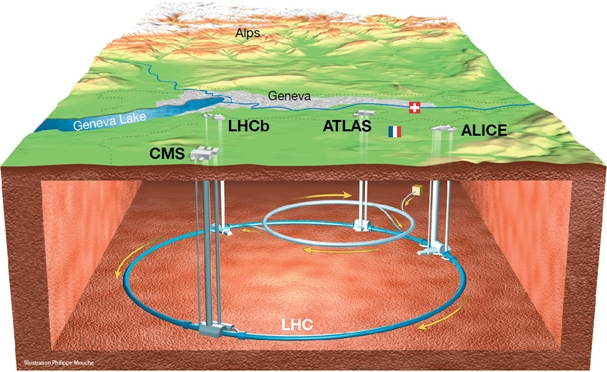
\includegraphics[width=0.9\linewidth]{images/LHC.jpg}
        \caption{A visual representation of the LHC at CERN. Above ground the four biggest particle detectors can be seen. Taken from \cite{CERN_official}.}
    \label{fig:LHC}
\end{figure}

There are four collision locations along the LHC, corresponding to the positions of four massive particle detectors, and therefore four experiments. Tens of millions of collisions take place every second at those locations, creating a dense particle plasma, the same that is speculated to have been present just seconds after the Big Bang occurred.

\subsection{ATLAS}
The ATLAS (A Toroidal LHC ApparatuS) experiment\cite{aad2008atlas} at CERN  investigates a wide range of physics, from the search for the Higgs boson to extra dimensions and particles that could make up dark matter.

\begin{figure}[t]
    \centering
    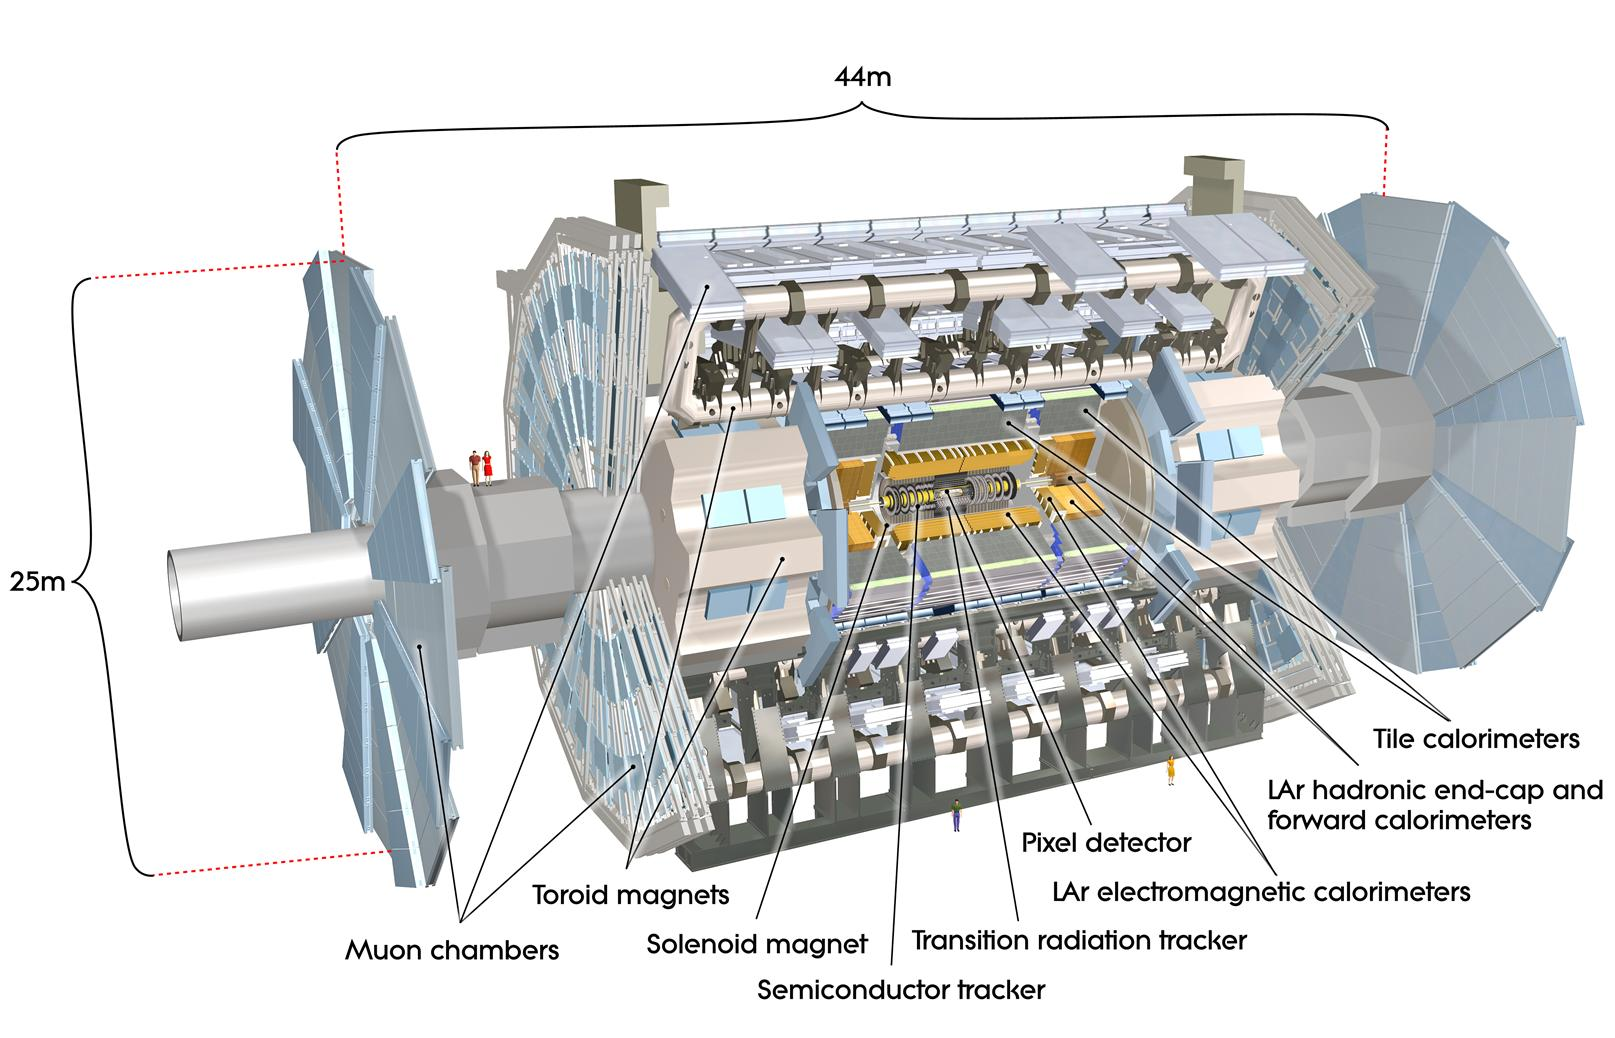
\includegraphics[width=1\linewidth]{images/atlas-detector.jpg}
    \caption{A visual representation of the ATLAS detector at CERN. Reference \cite{CERN_official}.}
    \label{fig:atlasdet}
\end{figure}

The ATLAS detector, shown in figure \ref{fig:atlasdet}, is one of the two general-purpose detectors at the LHC. Inside of it, six different detecting subsystems arranged in layers around the collision point record the path, momentum, and energy of the particles, allowing them to be individually identified and then try to reconstruct what was created back at the collision point.

\subsection{The ATLAS trigger system}\label{ch:trigger}
The interactions in the ATLAS detector create an enormous flow of data. To digest the data, ATLAS uses an advanced trigger system to tell the detector which events to record and which to ignore. Complex data-acquisition and computing systems are then used to analyse the collision events recorded.

Via two levels of filtering: an online trigger (as soon as the event has been recorded) and one offline (after the event has been saved), around 1000 events are being selected as interesting and possibly containing new physics out of the 40 million ones produced per second. %Jet algorithms, described in chapter \ref{ch:reconstruction} aid greatly to that.

Those events are the ones used as input data to the software that will be analysed in this report.
\section{Motivation}
This dissertation was a result of collaboration with the experimental particle physics group of the University of Edinburgh. The group suggested the project, aided in tailoring it as an HPC dissertation, and provided guidance throughout its duration. Also, a personal reason for the choice of this project is the student's ambition to pursue a PhD in experimental particle physics and the desire to comprehend the underlying physics.     

The luminosity of the LHC, which means the number of collisions that occur in a given amount of time, reaches new milestones with every new upgrade. This is done by increasing the number of particles that collide, or decreasing the diameter of the particle beams. This leads to more and more events to be analysed. There is no good reason creating those events if they cannot be processed properly and in time.

Jets are streams of particles emerging from the collision point and account for a considerable part of the analysis. In figure \ref{fig:jets1} jets are presented as light blue cones. Finding new ways to process jets quickly, namely jet reconstruction, is crucial for the future of experimental particle physics. The current dissertation project follows a performance analysis of two particle jet software packages.

The first one is FastJet, currently the most established one in the field and heavily used by the particle physics community. It is a C++ software package consisting of around 2 million lines of code and implementing many optimised jet reconstruction algorithms. The performance analysis of FastJet aimed to understand the reasons keeping it from running even faster, and also why it hasn't been parallelised yet. 


The second software package that was analysed follows a very different direction. It is a neural network that learns how to take as input data the output of different jet algorithms, and forms an unbiased opinion regarding the jet's substructure. It is written in Python with call to Keras, a high-level neural networks API, on top of Tensorfow, an open source machine learning framework. The performance analysis of this neural network aimed to discover any performance bottlenecks.

The university of Edinburgh experimental particles physics group is actively involved in the development of this software package.

\section{Chapters breakdown}

Chapter two, provides some physics insight to make the scope of the project more clear, while chapter three is an introduction to jet algorithms used by both software packages. 

Chapter four is a discussion regarding FastJet, and chapter five describes the performance analysis process that was followed.

Similarly, chapter six explains briefly what an adversarial neural network is and chapter seven introduces the jet substructure adversarial neural network. Chapter eight recites the performance analysis process for the neural network. 

In chapter nine, a discussion following both performance analyses takes place, and chapter ten is brief presentation of the findings.




\chapter{The Underlying Physics }
\section{Particle Collisions}

When trying to understand what the Universe is made of at a fundamental level, one can take ordinary matter and break it up into ever smaller and smaller pieces. But when that is over, very small constituents of matter will be found inside: everything around us is made of molecules, which are in turn made of atoms. Those can be broken into electrons and the nuclei. Every nucleus is composed of protons and neutrons. The two last are made up from quarks and gluons. 

That is not everything nature has to offer though. There are other more exotic particles out there that are not necessarily found inside ordinary matter. Thankfully, there is a convenient way to make a lot of what is possible for the universe to make: by taking advantage of special relativity. If enough energy is brought together in one location in space and time, a lot of what the universe allows can be created. The more energy there is available, the more massive the particles that can be created. See reference \cite{TheLHCmadesimple} for a more in-depth approach, written in everyday language.

This is exactly what is happening at the Large Hadron Collider. Physicists create collisions with as much energy as possible, by accelerating and colliding particles of ordinary matter. A representatino of a particle event can be seen in figure \ref{fig:jets1}. At the LHC protons are chosen because they exist in abundance and they are also heavy enough to radiate much less than electrons.

Since protons are so tiny, most of the times that they are shot at each other, they miss; but in the occasions they do collide, an avalanche of decays takes place. New particles are created from the existing energy, and then decay almost right away into other particles, again and again, until eventually stable particles are reached. The stable particles are the ones observed by the particle detectors.

\begin{figure}[H]
\centering
  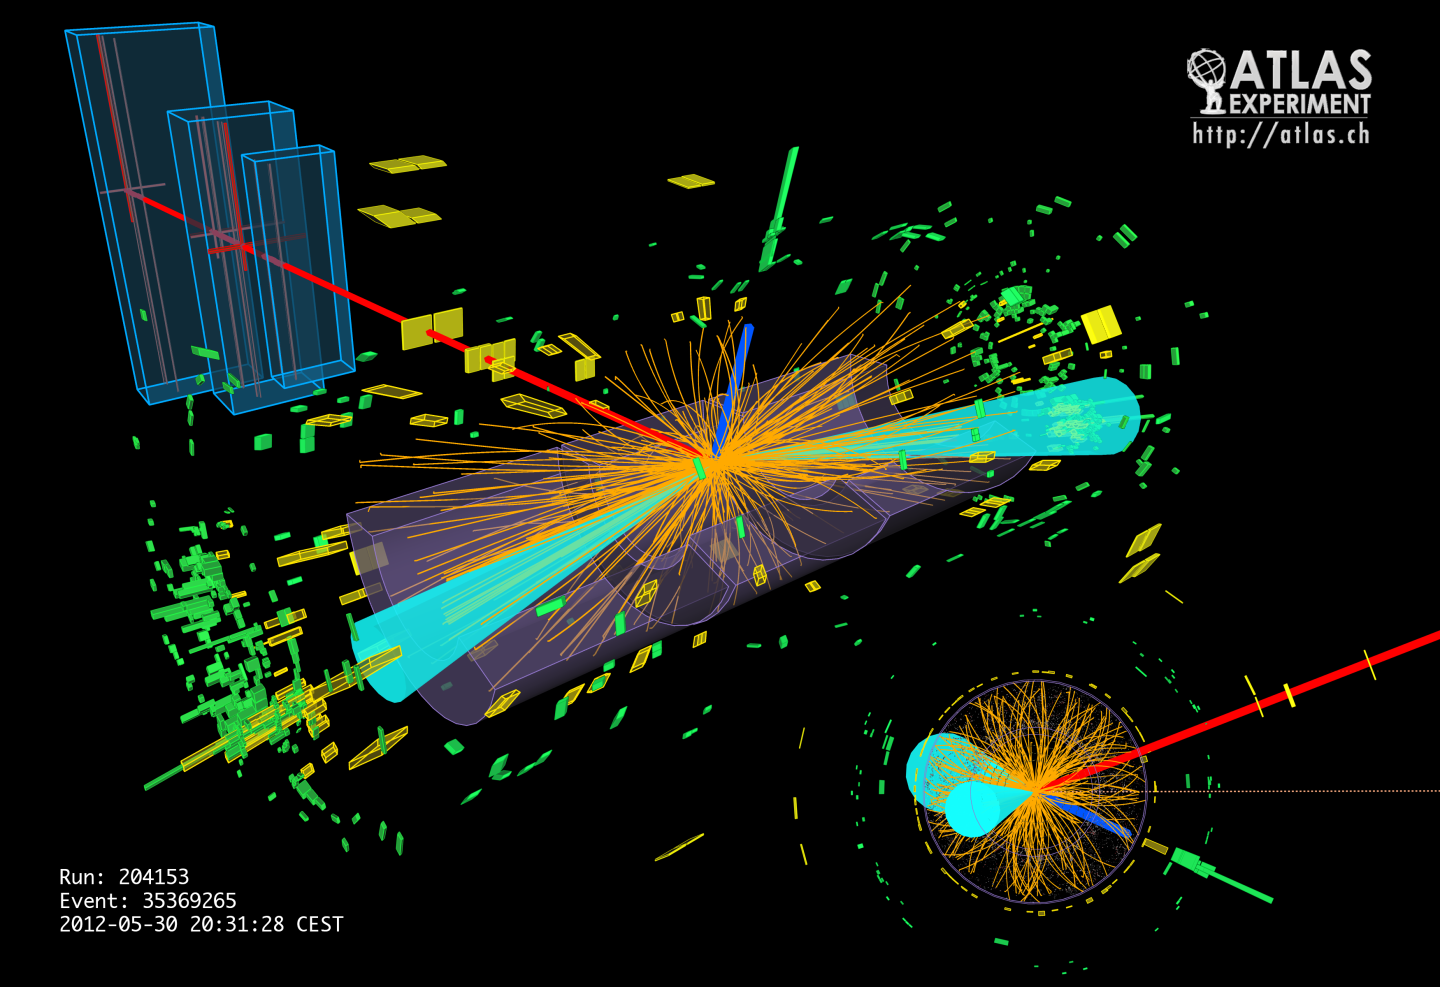
\includegraphics[width=\linewidth]{images/jets1.png}
  \caption{A visual representation of the particles flying out from the collision point. As can be seen, different types of particles are identified using different detecting systems (shown with distinct colours). The light blue cones represent particle jets. Reference \cite{aad2008atlas}.}
   \label{fig:jets1}
\end{figure}


\section{Particle Jets}\label{ch:particlejets}
The particles produced from the collisions fly out from the collision point in different ways depending on their type. Perhaps one of the most impressive and easily distinguishable observed structure is particle jets.  The formal definition of a jet is "a collimated spray of stable particles arising from the fragmentation and hadronisation of a parton (quark or gluon) after a collision" \cite{atkin2015review}. Essentially, a jet is a spray of particles, flying away from the collision point, forming a narrow beam. If the shape of a jet would be visualised it would look like one of the sky blue cones in figure \ref{fig:jets1}. This section aims to provide a basic understanding of that phenomenon.


Protons and neutrons are composite objects built out of three quarks, which are bound together by gluons. Quarks and gluons are assumed to be fundamental particles, meaning that they have no internal substructure. If one tries to pull a quark away from the rest they act like springs; the further and further a quark is pulled away, the greater the force with which it wants to “snap” back to the other quarks. The more the energy that is put to the system to get these particles further apart, the stronger and stronger the attractive force gets \cite{TheLHCmadesimplefreequarks,jetalltheway}.

In the case that someone insists on pulling the quarks further and further apart, this action will eventually require so much energy to be put to the system that, eventually, it will be enough for a new particle-antiparticle pair to be created out of the vacuum with it.%, rather than the quarks being pulled further apart.

This is the mechanism behind jet formation. In the collision points of LHC, every once in a while, there will be a huge jet of particles that fly off from the high-energy collision point. How do so many particles get together in one place? Because for a very brief moment, a high energy quark was created, and it began to pull all these particle-antiparticle pairs out of the vacuum. \cite{TheLHCmadesimplefreequarks,jets}.


\section{Boosted Particles and jet substructure}\label{ch:fatjet}

Physicists use \textbf{boost} to describe Lorentz transformations in relativity, meaning a conversion between two frames of reference that travel with different velocities. A \textbf{boosted particle} refers to a particle that travels at high speed through the laboratory. As the Large Hadron Collider at CERN operates at a very high beam energy, it is very common that the particles produced come out with very large velocity, thus boosted.

Typically, the heavy particles that interest physicists are not observed themselves, but decay into other particles, which in turn are captured by the particle detectors. The boost of the mother particle changes the way its decay products are observed in an experiment. 

To make this clearer, a heavy particle can be imagined decaying to two lighter blue particles, as in figure \ref{fig:boost}. If the heavy particle is at rest relative to the laboratory (figure \ref{fig:boost} left), because of conservation of momentum, the two decay products shoot off in opposite directions. If one is observed in the upper half of the detector, the other will be spotted in the lower half. On the other hand, if the heavy particle is boosted (figure \ref{fig:boost} right), the topology of the decay is quite different. Given a large enough boost, both daughter particles are emitted in the same direction. 

%To make this clearer, a heavy pink (with the solid circle) particle can be imagined decaying to two lighter blue (with the open circle) particles, as in figure \ref{fig:boost}. If the pink particle is at rest relative to the laboratory (figure \ref{fig:boost} left), because of conservation of momentum, the two decay products shoot off in opposite directions. If one is observed in the upper half of the detector, the other will be spotted in the lower half. On the other hand, if the pink particle is boosted (figure \ref{fig:boost} right), the topology of the decay is quite different. Both daughter particles are emitted in the same direction. 


For sufficiently large boost, both daughter particles will be very close together in the detector. If a boosted particle decays into quarks and anti-quarks their jets will overlap, up to the point where one can no longer distinguish the individual jets. As a result, the whole decay fuses into a single jet with substructure, meaning that it consists of more than one or more subjets. These jets are called  "fat" jets \cite{boosted}.

\begin{figure}[H]
  \centering
  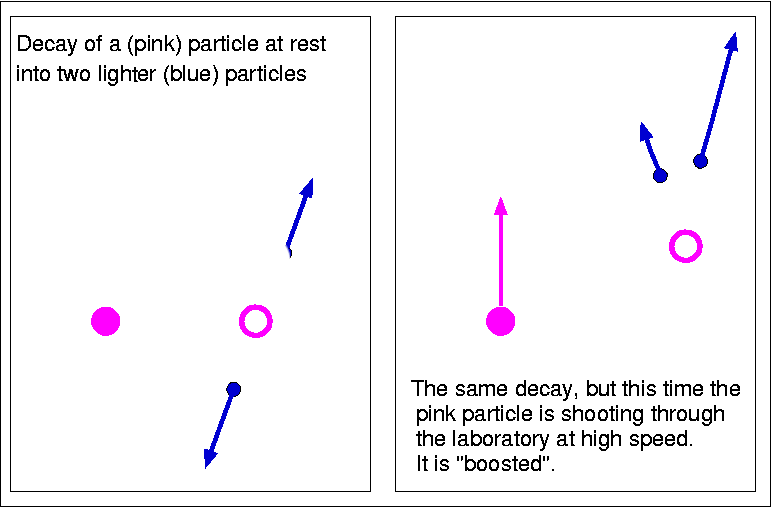
\includegraphics[width=\textwidth]{images/boost.png}
  \caption{A heavy pink (with the solid circle) particle decays to two lighter blue (with the open circle) particles. If the heavy pink particle is at rest relative to the laboratory (figure \ref{fig:boost} left), because of conservation of momentum, the two decay products shoot off in opposite directions. If one is observed in the upper half of the detector, the other will be spotted in the lower half. On the other hand, if the heavy pink particle is boosted (figure \ref{fig:boost} right), the topology of the decay is quite different. Both daughter particles are emitted in the same direction. Reference \cite{boosted}.}
  \label{fig:boost}
\end{figure}

The experiments only detect jets, but physicists are interested in the events that produced them. As a result, it is essential to be able to identify jets and reconstruct what produced them. This requires software packages such as FastJet. Algorithms, as well as being accurate, they need to operate rapidly to cope with the number of events. In the next chapter the algorithms implemented by FastJet are discussed.


\begin{comment}

\section{Boosted Higgs Analysis} \label{ch:higgs_analysis}
The Higgs boson's existence was confirmed back in 2012 by both the ATLAS and CMS experiments. (Un)surprisingly, the Higgs analysis did not stop there. There is currently a huge ongoing research studying a variety of its decays, hunting possible heavier charged Higgs bossons and much more.

Since the Higgs boson requires an enormous amount of energy to be produced, it often happens that it is created with a lot of Kinetic energy or, alternatively said, boosted.

\end{comment}



\chapter{Jet Algorithms}\label{ch:reconstruction}
A big part of the data analysis process at the ATLAS trigger system revolves around particle jets. Usually, when working with particle jets, the first action taken is to identify particles that belong to the same jet, namely jet reconstruction. This can provide a link between the observed stable particles and other particles too short-lived to be detected.

%This indirect detection also helps physicists infer properties of those particles, like their mass and spin. Also, through different jet reconstruction methods, physicists measure the total energy before and after a collision in the detector. If it is not what the theory predicts, this could lead to further understanding of physics, beyond the current theories \cite{atkin2015review,hodgkinson2008missing,JetReconstructionAlgorithms}.

Algorithms implementing jet reconstruction are discussed in the first half of this section. These algorithms are the ones chosen for the FastJet software and its performance analysis in chapters \ref{ch:fastjet} and \ref{ch:workfastjet}.  

After the initial jet reconstruction phase, more specialised methods can be applied. One example, jet substructure analysis, is discussed in the second half of this section. Boosted jets, that are comprised of two or more smaller jets (as explained in subsection \ref{ch:fatjet}), are being identified in order to improve the jet reconstruction accuracy. The output of these algorithms is being used as input for the jet reconstruction adversarial neural network discussed in chapters \ref{ch:chann} and \ref{ch:jsann}.


\section{Jet Reconstruction Algorithms}\label{ch:seq_alg}
    A jet reconstruction algorithm is a set of rules that projects a set of particles onto a set of jets \cite{cacciari2012fastjet}. There are various jet reconstruction algorithms developed over the years, aiming to define the kinematics and shape of the jets. There are two main categories: cone algorithms and sequential clustering algorithms.

    Before analysing those two categories, it is worth discussing a property of jet algorithms called Infrared (IR) safety. For algorithms that are IR safe, if two events are almost identical with the exception of the addition of a low energy (soft) particle to one of them, the jets that are reconstructed from each event should also be almost the same. This means that very low energy particles should not essentially contribute to the clustering. A good reconstruction algorithm should therefore be IR safe \cite{algorithms_irc}.% because it is undesirable for fine-details of the detector to have have significant impact on the clustering output .
    
    \subsection{Cone algorithms}
    Cone algorithms assume that particles in jets will show up in conical regions and thus they cluster based on geometry, resulting in jets with rigid circular boundaries (figure \ref{fig:cone}). Differences between various cone algorithms have to do with the strategy taken to search for the stable cones and the procedure used to deal with cases where the same particle is found in multiple stable cones\cite{cacciari2012fastjet}.

\begin{figure}[H]
    \centering
    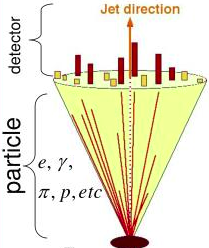
\includegraphics[width=0.4\linewidth]{images/cone_alg.png}
    \caption{Graphical representation of a jet reconstructed using a cone algorithm. All the particles (red lines) included in the conical region are considered part of the jet.}
    \label{fig:cone}
\end{figure}

        In the past, cone algorithms were preferred by physicists as they were more intuitive and easier to implement in a computationally cheap way. However, in the last few years, cone algorithms have tended to be used less and less due to the fact that they are considered to be IR unsafe and that they contain non-physical constants (arbitrary parameters that do not have a meaning in nature). 
        
        Because of their lack of usage, in this project no cone algorithms were selected to work on. This category is presented here for the sake of completeness. 

    \subsection{Sequential Clustering Algorithms}\label{ch:seq}

    Algorithms that belong in the second category, sequential clustering algorithms, assume that particles within jets will have small differences in their momenta and, thus, group particles based on that. 

    Usually the two particles whose momenta are closest together are identified and merged together into one particle. Then the procedure is repeated over and again, until some stopping criterion is reached. The stopping criterion is usually the radius parameter (\textbf{R}), which roughly determines the final size of the jet. The main difference between the various sequential recombination algorithms is their particular choices of distance measure and stopping criterion.  

    Sequential clustering algorithms utilise more physical constants than cone algorithms, and are also IR safe. In the past, algorithms of this type were not favoured as much by physicists because they had slow computational performance. As time progresses, the more optimised versions of algorithms, have resulted in sequential clustering algorithms dominating the particle physics community.
    
    The two most commonly used sequential clustering algorithms are: the anti-$K_t$ and Cambridge/Aachen. The former does a very good job at resolving jets but it is rather difficult to use its results for studying jet substructure. The latter does a good job at resolving jets but its results are much easier to decluster and look for further substructure \cite{atkin2015review}.

\section{Jet substructure algorithms}\label{ch:sub_alg}
As described in chapter \ref{ch:fatjet}, often two or more jets coming from a boosted particle can be so close together that jet reconstruction algorithms find it hard to distinguish between them. One way to deal with this is to treat them as one single fat-jet and apply substructure methods at a later stage. There exists a category of jet variables representing the probability that a particular jet has substructure or what that substructure may be.

\subsection{Substructure variables}\label{ch_sub}

%\verb|https://arxiv.org/pdf/1203.4606.pdf|
\subsubsection{\texorpdfstring{N-subjettiness (${\tau}_{N}$)}{N-subjettiness tau 21)}}
The N-subjettiness variables $\tau_{N}$ are continuous observables related to the subjet multiplicity. Intuitively, the variables can be thought of as answering the question: “How much does this jet look like $N$ different subjets?” \cite{ccetin2012jet}.

The variable $\tau_{N}$ is calculated by re-clustering the constituents of the jet with the kt algorithm and requiring $N$ subjets to be found. Using this definition, this substructure variable describes how well the substructure of the jet is described by $N$ subjets by assessing the degree to which constituents are localised near the axes defined by the kt subjets \cite{ccetin2012jet}.
\subsubsection{\texorpdfstring{$D_2$}{$D_2$}}
$D_2$ investigates how a jet's constituents spread in momentum space and outputs a distribution of probability of this jet consisting of subjets \cite{lectured2}. 

\chapter{FastJet}\label{ch:fastjet}
The first of the two software packages chosen for performance analysis is FastJet \cite{fastjet_site}. It is the most widely used jet reconstruction software, and for good reasons. An extensive range of jet finding tools and a number of jet substructure utilities, considered in chapter \ref{ch:reconstruction}, are implemented. FastJet is written using C++ and consists of around two million lines of code spread in one thousand different files. Its capabilities are vast, and extend way beyond the scope of this project.

\section{Why FastJet}\label{ch:whyfj}
So, what is it that makes FastJet so loved by the physics community? First of all, its simple interface. All the tools and methods incorporated by FastJet are easily accessed and can be used by writing a few lines of code. Proof of that is the  example code provided in section \ref{ch:fjexample}. Secondly, its flexibility and insensibility. The software is written in such a way that different parts of it can fit together like puzzle pieces and be combined however the user wants. Moreover, there is a very active community of FastJet contributors amongst physicists, implementing new jet algorithms. 

%The difficulty that arises, however, is that at hadron colliders, clustering is often performed with several hundreds or even thousands of particles. Given N particles, there are N(N - 1)/2 dij distances to calculate, and since one must identify the smallest of these O(N2) distances at each of O(N) iterations of the algorithm, original implementations of the kt algorithm [11, 12] involved O (N3) operations to perform the clustering. 

%In practice this translates to about 1 s for N = 1000. Given that events with pileup can have multiplicities significantly in excess of 1000 and that it can be necessary to cluster hundreds of millions of events, N3 timing quickly becomes prohibitive, all the more so in time-critical contexts such as online triggers. 

The third reason that makes FastJet so popular, which may also be the most important, is its speed. The truth is, a few of the FastJet algorithms can be naively implemented in just several lines of code. The difference rises, when the clustering has to be performed with several hundreds or even thousands of particles. 

Simple implementations scale as $O(N^3)$, essentially calculating the smallest distance between any two particles for a number of iterations. These implementations, when put against the vast amount of events to be processed, struggle to keep up. Even more in time sensitive environments, like the ATLAS online trigger system. 

The algorithms included in FastJet, on the other hand, make use of symmetries that exist when calculating the distance between two particles, and use optimised versions of the numerical equations so that some parts of them are constant and do not have to be recalculated on each step. Moreover, many constrains implied by the geometry of the problems are taken into account to make the computations less expensive. Finally, where possible, FastJet utilises external libraries, for example Computational Geometry Algorithms Library (CGAL). Taking into account everything mentioned in this paragraph, FastJet manages to achieve an $O(N^{2}* ln(N))$ scaling \cite{cacciari2012fastjet}.

In order to understand the magnitude of the improvement FastJet provides, for 1000 particles, a naively implemented $O(N^3)$ scaling algorithm would take around $1s$ to calculate the result. On the other hand, FastJet's $O(N^{2}* ln(N))$ scaling can compute that in milliseconds, making it almost 1000 times faster.


\subsection{Choice of algorithmic strategy}\label{ch:fjstrategy}
FastJet contains different ways of implementing each algorithm. Depending on the number of particles and the radius parameter R (how big the final jet should be), FastJet has the freedom to choose which implementation of the algorithm is the most appropriate to use. The user can pass an extra algorithmic \textit{strategy} argument to the clustering function, requesting a specific strategy, but this just acts as a guideline and FastJet is free to ignore it.

Figure \ref{fig:fjstrategy} shows for two clustering algorithms, the anti-kt and Cambridge, the implementation strategy that will most probably be selected depending on the number of particles and the radius (R). The choice of strategy is done for performance reasons. The optimal strategy may vary depending on the system FastJet is being ran on. That is not taken into account of by FastJet though.

\begin{figure}[H]
    \centering
    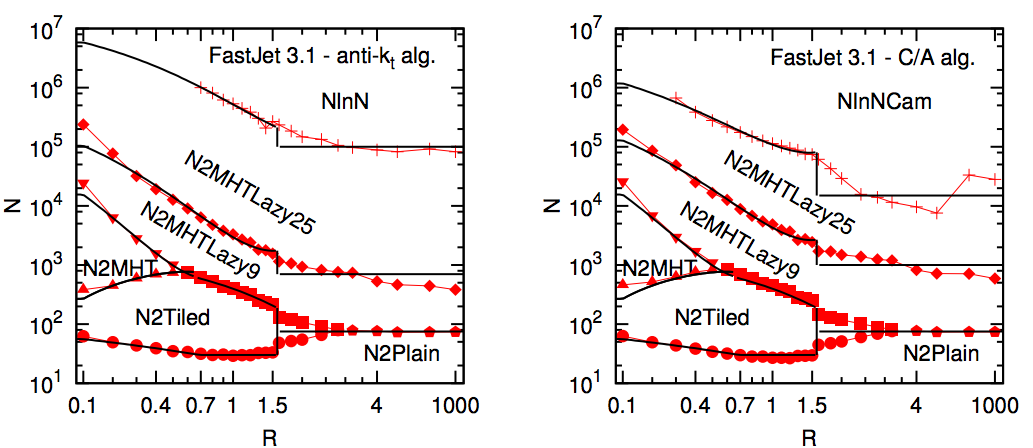
\includegraphics[width=\linewidth]{images/fjstrategy.png}
    \caption{Transitions between chosen strategies in the plane of particle multiplicity N and radius R. The red lines with symbols indicate the measured transitions, while the black solid lines are the
approximate transitions used for the chosen strategy. The left plot is for anti-kt and the right for Cambridge. Taken from \cite{cacciari2012fastjet}.}
    \label{fig:fjstrategy}
\end{figure}


\subsection{Tiled strategy}\label{ch:tiled}
Of the FastJet strategies mentioned, one will directly concern the performance analysis of chapter \ref{ch:workfastjet}, and is thus explained here. When a sequential clustering algorithm iterates through all the particles of the event to find their nearest neighbour, it is rather inefficient to examine the distance to any other particle. For some of them, it is already known that they are far away.

Optimised versions of these algorithms separate the particles in tiles. Depending on the definition of distance for each algorithm, particles that are closer together are put in the same tile. When looking for the nearest neighbour, it is only necessary to examine the particles in the same and neighbouring tiles. Grouping particles in tiles is an extra computational step that has to be taken, but it is done only once at the start of the algorithm and as pairs of particles are merged, it just has to be kept updated.

\section{Installing FastJet}\label{ch:fjtech}
FastJet is available under the GNU public license and can be downloaded from the official FastJet website(\cite{fastjet_site}. In order to be used, FastJet should first be installed on a system. The process includes utilising a configure file, that when run produces a Makefile. In turn, the Makefile can be used to compile the software. The installation process is pretty much straightforward and takes roughly three and a half  minutes on Cirrus\footnote{Cirrus is discussed in section \ref{ch:cirrus}}.  

The default compiler is GNU, the default compiler optimisation flag is -O2, and library linking is dynamic. Those can be changed through arguments on the configure phase of the installation. For example, in order to use the Intel compilers and the -O3 flag, the user can add to the first line:

\begin{lstlisting}
     CC=icc CXX=icpc CXXFLAGS=-O3 CFLAGS="-O3"
\end{lstlisting} 

Many of the algorithms that can be implemented by FastJet are not included in the FastJet built-in functions, but in an open source add-on package called FastJet Contributions \cite{fjcontrib}. The procedure to install this add-on is almost identical to the one followed to install the core FastJet software. The sole difference is that an extra argument has to be passed while configuring, pointing the location of the original FastJet configure file.

\section{Using FastJet}
After the installation, in order to use FastJet, the user is able to write their own C++ code, including the appropriate header file. Then the user's code can be linked to the FastJet libraries and compiled. 

FastJet heavily utilises classes and std:vectors. For basic usage of the software there exist three core classes PseudoJet, JetDefinition and ClusterSequence. For more detailed explanation, refer to chapter 3 of the FastJet manual \cite{cacciari2012fastjet}. Following the definitions a simple example of FastJet usage follows, in order to aid the understanding of FastJet usage.

\subsection{FastJet core classes}
\subsubsection{PseudoJet}\label{ch:pseudojet}
All jets, as well as input particles to the clustering, are PseudoJet objects. The PseudoJet class provides a jet object with a four-momentum and some internal indices to situate it in the context of a jet-clustering sequence.

\subsubsection{JetDefinition}
The class JetDefinition contains a specification of how jet clustering is to be performed. Usually, a "jet definition" instance includes the jet algorithm name, the radius R,  possibly the strategy, and the recombination scheme. 

The Recombination scheme is the way the four-momentum of pseudojets will be combined when these are merged. It can vary from simple addition of the individual components to complex functions.


\subsubsection{ClusterSequence}
To run the jet clustering, the user is required to create a ClusterSequence object. The ClusterSequence class carries out jet-clustering and provides access to the final jets.

\subsection{FastJet example Code}\label{ch:fjexample}
From the bellow example code, in lines \ref{line:A} to \ref{line:B} jets are defined, while in lines \ref{line:C} to \ref{line:D} they are passed to the algorithm.


\lstinputlisting[language=C++,escapechar=|]{codes/example_code.cc}

In order for the code to be compiled, the directory of the installed FastJet files should be pointed out by:

\begin{lstlisting}
g++ example.cc -o example \
     `fastjet-install/bin/fastjet-config --cxxflags --libs --plugins`
\end{lstlisting}

\chapter{Performance analysis of FastJet}\label{ch:workfastjet}
This chapter describes the steps followed for a performance analysis of FastJet. Initially the installation process on the two computing systems, Cirrus and ARCHER is discussed, followed by the set-up of the analysis framework. Then, the profiling process is explained and the results are examined. Finally, the last section of this chapter looks into some efforts that were made to speed-up FastJet and what the future may hold for it.

\section{FastJet on different Computing systems}
For the needs of this project, FastJet was installed on two computing systems, Cirrus and ARCHER. This section provides some basic information regarding those systems, and also any abnormalities in the process of installing FastJet on them.
\subsection{Cirrus}\label{ch:cirrus}
Cirrus was the main system that performance experiments were run on and it was selected for a number of reasons. It has modern Intel processors, provides the ability to choose between two compilers (GCC and Intel), allows for easy testing on the front-end but also for exclusive access to back-end nodes via the batch system, the software system is fairly standard Linux, and the student was already familiar with it from the MSc courses. 

\subsubsection{Hardware}
Cirrus\cite{cirrus} was the main system that the analysis for FastJet was performed on. It is one of the EPSRC Tier-2 National HPC Services and consists of 280 compute nodes, each with 256 GB of memory, connected together by a single Infiniband fabric. Each node contains two 2.1 GHz, 18-core Intel Xeon processors. In total there are 10.080 cores in Cirrus. Since Cirrus' processors support hyperthreading, up to 72 cores can be used in a single node.
\subsubsection{Installation process}
The installation process on Cirrus was already included in subsection \ref{ch:fjtech} of chapter \nameref{ch:fastjet}. The reason for that is to provide a more pedagogical approach for FastJet to the reader. 

\subsection{ARCHER}\label{ch:fj-ARCHER}
The main motivation for using ARCHER was the availability of CrayPAT (which is discussed in section \ref{ch:craypat}). ARCHER, having three compilers (.,.,.) was more appealing for some performance tests, but its CPUs are older and it is it is rather non-standard in terms of the OS and setup.



\subsubsection{Hardware}
ARCHER \cite{ARCHER} is the UK National Supercomputing Service. It consists of 4920 compute nodes, each with 64 (a few nodes have 128) GB of memory. Each node contains two 12-core Intel Ivy Bridge series processors. In total there are 118.080 processing cores on ARCHER.

\subsubsection{Installation process}
ARCHER, being a CRAY machine, seemed like a good option in order to profile FastJet using CrayPat. Installing FastJet on ARCHER with the GNU compiler (which is the default FastJet compiler), ran smoothly. In order to use CrayPat for profiling though, the code in question should be compiled using the Cray compiler. As a result, an effort was made to install FastJet again, but this time, when executing the configure file, the Cray Compiler was chosen (PrgEnv-cray module is required in order to use the Cray compiler but it is loaded by default on ARCHER):

\begin{lstlisting}
./configure CC=cc CXX=CC --prefix=$PWD/../fastjet-install
make
\end{lstlisting}

A number of GNU compiler flags are hard-coded into the compiling process. These flags are incompatible with the Cray compiler, and caused the compilation to fail.  As a workaround, the Cray wrapper on top of GNU compiler was used, so that the compiler flags would be compatible:
\begin{lstlisting}
module swap PrgEnv-cray PrgEnv-gnu

./configure --prefix=$PWD/../fastjet-install
make
\end{lstlisting}

On ARCHER every library is by default linked statically. As it turns out, some of FastJet libraries cannot be linked statically and caused the compilation to fail. From ARCHER documentation, a way to link libraries in a dynamic way was tried: 

\begin{lstlisting}
./configure CC=cc CXX=CC CRAYPE_LINK_TYPE=dynamic --prefix=$PWD/../fastjet-install
\end{lstlisting}

This still produced errors, and the compilation failed. At this point, considering that ARCHER was not the main system to be used for the dissertation project, it was decided to stop the effort and focus the performance analysis using Cirrus.

\section{Setting up the analysis}
\subsection{Choice of algorithms}
As described in the previous chapter, FastJet provides the opportunity to perform several different types of analysis. Naturally, for the scope and length of this project, it seemed sensible to make a selection of a few of them. Therefore, two jet reconstruction algorithms (chapter \ref{ch:seq_alg}), Cambridge/Aachen and the anti-$k_t$, were chosen to perform the analysis on. The decision for these two algorithms was based on the fact that they are considered the best on jet clustering by the physics department of the university of Edinburgh, are widely used, and any possible performance improvement on them would have a considerable impact on the community. 


\subsection{Choice of input data}
Having chosen the algorithms, it was then time to find appropriate and meaningful input data. 

A large input file consisting of sixty thousand particle collision events, and a size of 220MB, was supplied by the particle physics department for the needs of the project. Every event consists of around 100 particles. Particles per event is an important parameter for the reconstruction and it greatly affects the algorithmic strategy of FastJet.

\subsection{Writing the test code}\label{ch:testcode}
For the purpose of the project a C++ program was written, utilising FastJet's classes and algorithms, in order to analyse their performance. The program was separated in three main functions:
\begin{itemize}
    \item \textbf{read input data:} Stores all the particles per event in a vector of pseudojets.    
    \item \textbf{perform clustering:}
    Loops through all the events, and for each one of them, performs the jet reconstruction according to the parameters set.
    \item \textbf{print reconstructed jets:}
    Prints to the screen all the reconstructed data.
\end{itemize}

The writing of the program was greatly aided and influenced by the provided FastJet examples; nevertheless some considerable work had to be done to tailor it for the needs of the project. The test code in its entirety can be found in Appendix \ref{ch:test_code_code}. 

\subsection{Performance analysis framework}
At several different points of the analysis, changes were attempted to the default behaviour of FastJet either to deepen the understanding of the software or to check a speculation. These changes could be different compiler flags, different compilers, altering the test code, or even modifying the FastJet libraries. Usually, each change was followed by measuring the performance of FastJet under the new conditions.

To make sure that the right results were still produced after each modification, a reference output file containing the correct results was created. After each run, the newly created output file was compared to the reference output file. In some occasions, changes would create an output file different to the reference output file, while still being correct; for example the jets would just be out of order. Those were treated separately.

Every performance measurement, unless explicitly stated otherwise, was run on the back-end of Cirrus and is the average of at least 5 runs. To achieve accuracy of the timing measurements, c++11's class std::chrono was used. Finally on\textbf{}ly the time spent in the perform function was timed. This is because, the time spent during IO is not relevant to the scope of the project.



\section{Choice of compiler and compiler optimisation flag}

After getting FastJet up and running, writing a test case, and getting the input data, some initial tests were run in order to gain a basic understanding of FastJet's performance.

Cirrus has two compilers installed, GNU and Intel. FastJet and the test code were compiled with each one of the compilers (GNU version  4.8.5, Intel 17) and optimisation flag (O0, O1, O2, O3, Ofast\footnote{Flag -Ofast enables all optimisation of O3, and also lets the compiler ignore finite precision of floating point numbers. This allows more optimizations, but can cause inaccuracies in the results due to rounding errors.}).

The process was repeated for two algorithms, anti-$k_t$ and Cambridge. The results can be seen in figure \ref{fig:flags}. The performance of both compilers for both algorithms is almost identical, although the GNU compiler performs slightly better. There is a big improvement between the first two compiler optimisation flags, and optimisation flag O2 performs better than O3. The reason for that may be that O3 flag optimizations increase code size (for example more aggressive loop unrolling), which can sometimes lead to slower performance. 


\begin{figure}[H]
    \centering
        \begin{subfigure}[b]{0.3\textwidth}
        \centering
    \end{subfigure}
    \hfill
    \begin{subfigure}[b]{0.3\textwidth}
        \centering
        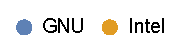
\includegraphics[width=0.6\textwidth]{images/flagsleg.eps}
    \end{subfigure}
    \hfill
    \begin{subfigure}[b]{0.3\textwidth}
    \centering
    \end{subfigure}
    
    \begin{subfigure}[b]{0.48\textwidth}
        \centering
        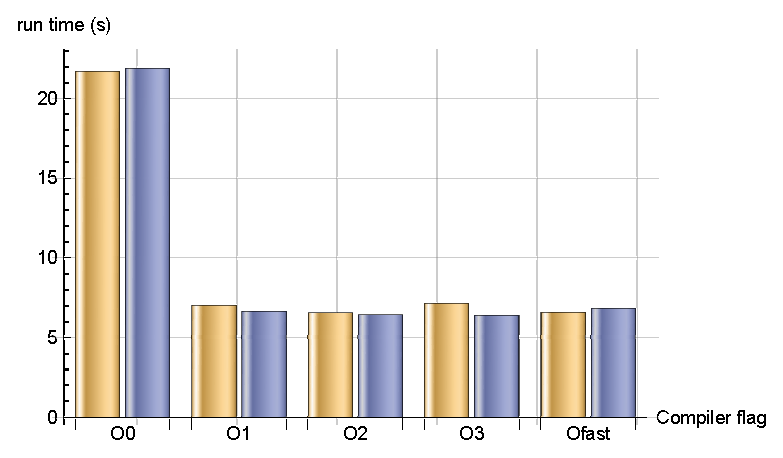
\includegraphics[width=1.2\textwidth]{images/flagskt.eps}
        \caption{Anti-$k_t$}
    \end{subfigure}
    \hfill
    \begin{subfigure}[b]{0.48\textwidth}
        \centering
        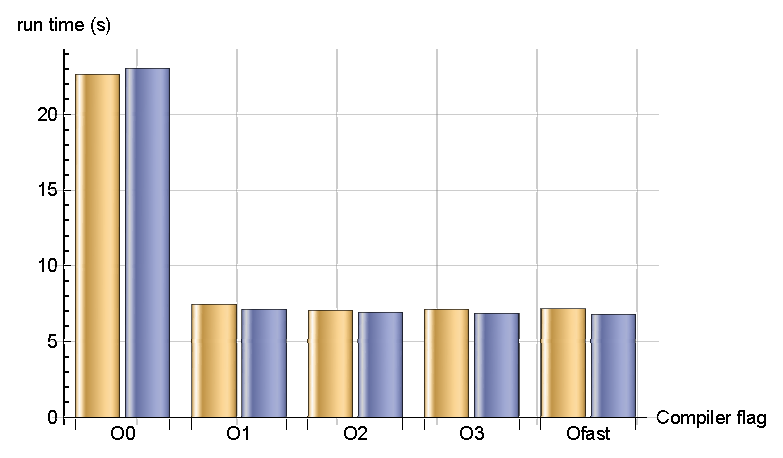
\includegraphics[width=1.2\textwidth]{images/flagscam.eps}
        \caption{Cambridge}
    \end{subfigure}
    \hfill
    \caption{Run-time versus compiler optimisation flag for two compilers. Each plot represents a different algorithm}
    \label{fig:flags}
\end{figure}

\section{Finding the most suitable profiler}
Profiling is the process of measuring an application or system. Profiling tools can provide information for different parts of the application: functions call, memory usage, CPU load, and resource usage. Two types of profiling that are worth mentioning are statistical profiling and tracing. Statistical Profiling is a way to profile an application by taking samples of the execution state during regular intervals at run-time. Tracing tools on the other hand generate results based on a detailed log of events within the program.

The initial experiments described in the previous section, provided an idea of FastJet's performance. The next step was to pinpoint which of the numerous FastJet functions are called with the current choice of algorithms, number of particles per event, and radius R. Afterwards, inspect which lines of code and loops are the most computationally expensive. 

\subsection{GNU gprof}

GNU Gprof is a statistical profiler for Unix based applications. Usually, the simplicity of usage it offers, makes it the fist choice when profiling software. GNU gprof version 2.25 which is installed on Cirrus was used. As per the usage instructions, FastJet software and the test code were compiled with the -pg flag. 

Interestingly, the profiling result only accounted for a small fraction of run-time. Only the time spent in the test code, but not in any FastJet functions, was accounted for. After seeking advice from the relevant gprof documentation, it was realised that GNU gprof cannot profile libraries that are linked dynamically. 

From Cirrus documentation, the command ldd + <executable> was used to check which libraries were linked dynamically. Indeed, a number of FastJet objects showed up as being linked dynamically. The -Bstatic flag followed by the full path of those libraries was used when compiling to force a static linking.

This time, the result of gprof accounted for the whole run-time and the FastJet functions explicitly called by the test code were shown. Nevertheless, profiling did not show the percentage of time spent in any other internal functions of FastJet. It was then decided that it was better, in terms of time-management and to keep to the right track for the project, to try and use a different profiler.


\subsection{CrayPat}\label{ch:craypat}
The Cray Performance Measurement and Analysis Tools (CrayPat) are a suite of utilities that capture and analyse performance data generated during the execution of a program on a Cray system\cite{craypat}. It can be used for both statistical profiling and tracing. CrayPAT is a very powerful tool that is well documented and frequently used by EPCC staff. It seemed to be a good candidate to provide insights on FastJet at the time. 

CrayPat requires that the source code is compiled using the Cray compiler on a Cray machine in order to succeed in profiling the software. However, as discussed on subsection \ref{ch:fj-ARCHER}, a number of difficulties arose while trying to install FastJet on ARCHER with the Cray Compiler. As a result, it proved more time consuming than intended to get any profiling results using CrayPat. Once more, to save time, it was decided to choose a different profiler.

\subsection{Gperftools}
A good alternative to the previous profilers was the gperftools profiler\cite{gperf}, a set of tools for statistical performance profiling and memory checking. Although, again, the profiling process was not trouble-free, the results were satisfactory. 

As gperf tools profiler is not currently installed on Cirrus and due to the limited privileges of the student's account, there was not a straightforward way to install in. As a result, it was installed in a Singularity container and copied to Cirrus. 

\subsubsection{Creating a singularity container image}\label{ch:singularity}
A container image is a lightweight, standalone, executable package of software that includes everything needed to run an application: code, runtime, system tools, system libraries and settings. Conveniently, Singularity\cite{kurtzer2017singularity}, a type of container, is already installed on Cirrus. 

First of all, one has to create the singularity image on a system with administrative privileges, through a singularity recipe. The student's laptop was chosen for that purpose. A singularity recipe is a text file, containing the necessary information for the image to be built. A singularity recipe was created, greatly influenced by the singularity documentation.

\lstinputlisting[language=bash]{codes/singularity_recipe.sh}

In order to create the image, the following command was executed.

\begin{lstlisting}[language=bash]
sudo singularity build --writable image_name.sing recipe.def
\end{lstlisting}

Where, the flag --writable provides the possibility for the image to be changed in a later time. The next step was to copy the newly created image to Cirrus. Having done that, the following command initiates an interactive shell inside the image, allowing the the software installed in it to be used.

\begin{lstlisting}[language=bash]
module load singularity
singularity shell image_name.sing
\end{lstlisting}

\subsubsection{Profiling}\label{ch:gerf1}
There exist two main ways to profile software with gperf tools. Both are just different alternatives of starting the profiler before the executable to be profiled. The first option is to recompile FastJet and the test code with the flag -lprofiler, and the second to set the environmental variable LD\_PRELOAD accordingly. Bellow, the second method, which was followed, is explained. The environmental variable CPUPROFILE is set to be the output file of the profiling.

The process to follow in order to profile the code on Cirrus is: 
\begin{lstlisting}[language=bash]
module load singularity
singularity shell <path_to_the_singularity_image> #Enter an interactive shell where gperf tools are installed

#LD_PRELOAD allows the profiler to be executed prior to the software
#CPUPROFILE sets the output file of the profiling
LD_PRELOAD=/usr/lib/libprofiler.so CPUPROFILE=./profiling_result.prof ./<path_to_executable> #in one command
\end{lstlisting}

After that, the profiling of the software will start. Upon completion, a terminal output will read:  PROFILE: interrupts/evictions/bytes = \textit{"some number"}\\ An output file will be created to where CPUPROFILE is pointing at. 

\subsubsection{Processing the output}

The output file from the profiling, can be used in order to create more human readable profiling results. The command to do that is:
\begin{lstlisting}[language=bash]
google-pprof [Output Type] [Granularity] [Display] ./profiling_result.prof > output.file
\end{lstlisting}

where:
\begin{itemize}
    \item \textbf{Output} denotes the output file type (text, pdf, gif, etc)
    \item \textbf{Granularity} is what nodes will represent (addresses, lines, functions, files)
    \item \textbf{Display} provides a few possibilities on the nodes are shown.
\end{itemize}

For example a user friendly output saved as pdf (similar to the one shown in figure \ref{fig:gperfnatikt}) can be requested by using:
\begin{lstlisting}[language=bash]
google-pprof --pdf --functions ./profiling_result.prof
    > output_file.pdf
\end{lstlisting}

\subsubsection{Focused profiling}
The profiling process described until now, accounts for the whole run-time of the software. As this project focuses only on the clustering phase, a way was sought for selective profiling. Two ways were found.

The first one involved, making use of calls from the test code to the functions ProfilerStart() and  ProfilerStop(). For this to work out, the profiling was stopped at the start of the main function, started again right before the clustering function and stopped again afterwards. The header file <gperftools/profiler.h> has to also be included for the functions to work. 

The reader may have noticed that the contents of the singularity recipe file include the installation the GNU compilers. This is only necessary for the method that has just been described. The reason is that, once the header file of the previous paragraph is included in the source code, gperf tools must be installed on a system for the code to compile. Thus, the interactive shell is loaded prior to compiling.

The second way for selective profiling is much simpler, but was discovered a while after the first one. It involves profiling the whole run-time of the software and then using the clause \verb|--|focus=<desired\_function> while processing the output. This only performs the analysis for the <desired\_function>. There exist also the \verb|--|ignore clause with the opposite functionality.

\subsubsection{Profiling results} 
The profiling result of gperf tools was very informative. FastJet internal function calls are shown very clearly. The graph for the anti-kt and the Cambridge algorithms, focused only on the perform\_clustering function, can be seen on figures \ref{fig:gperfnatikt} and \ref{fig:gperfcamb} respectively. Each node represents a procedure. The directed edges indicate caller to callee relations. Each node is formatted as follows: class name, function name, local percentage, cumulative percentage.

\begin{figure}[H]
    \centering
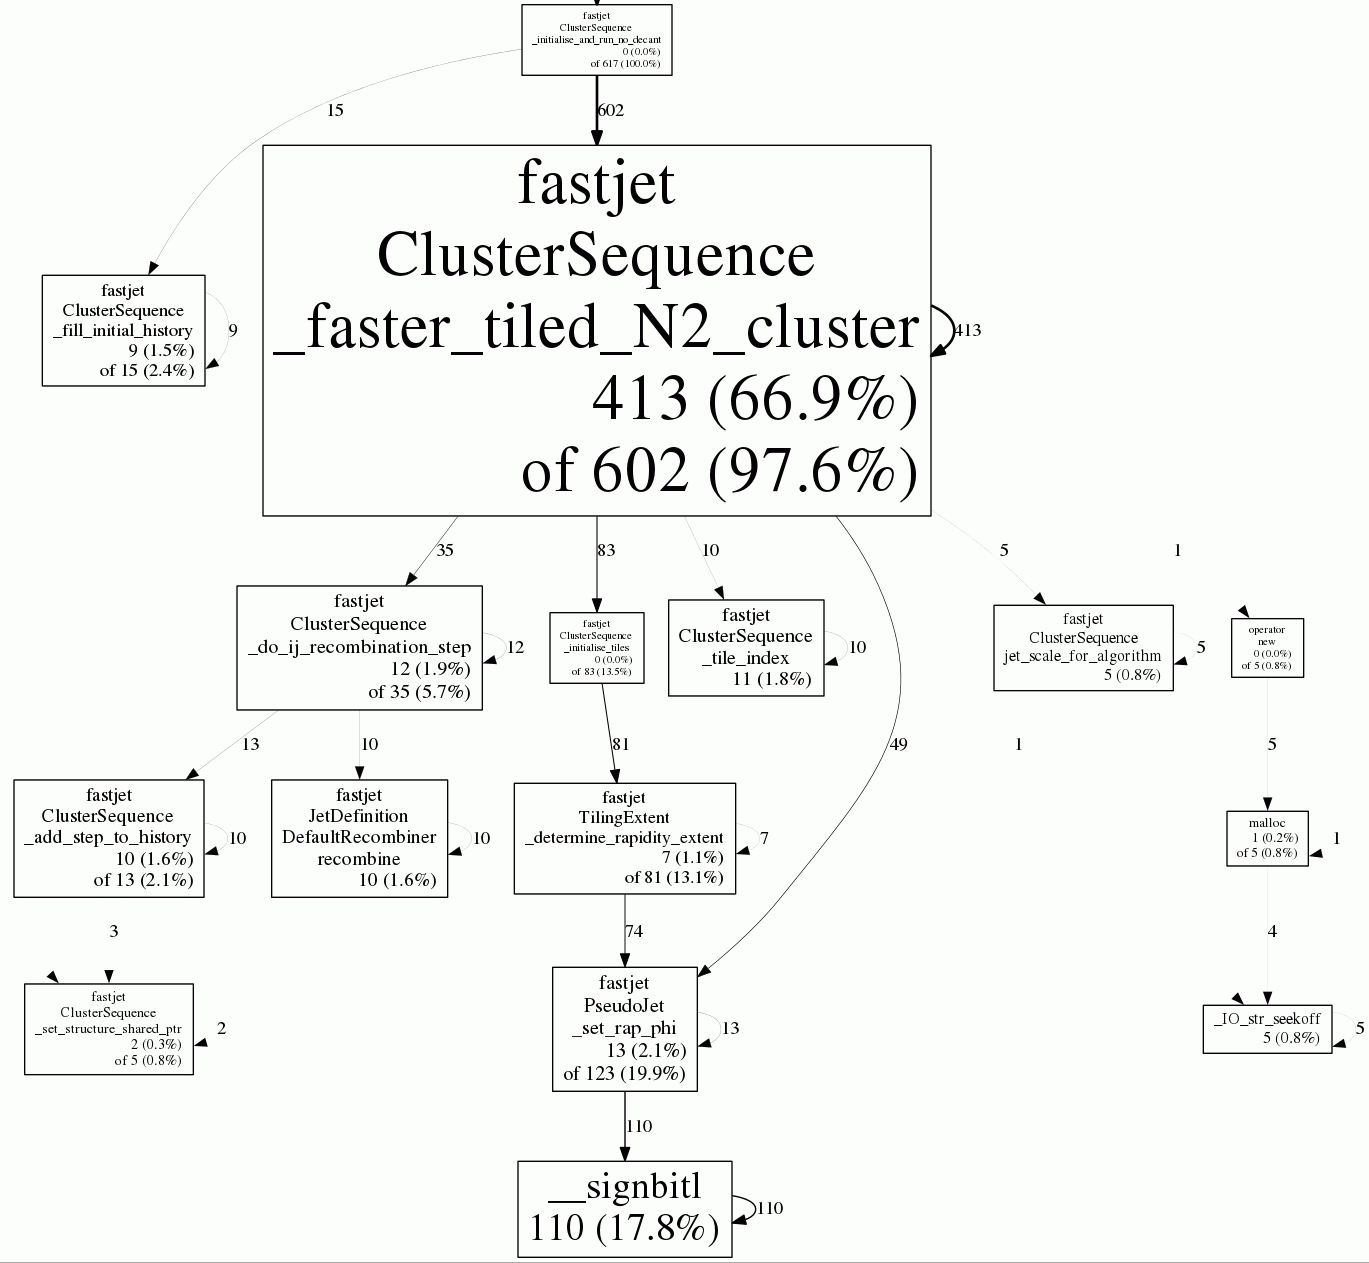
\includegraphics[width=1\linewidth]{august2_antikt.jpeg}
    \caption{Profiling result using gperf tools for the anti-kt algorithm, focused only on the perform\_clustering function.}
    \label{fig:gperfnatikt}
\end{figure}

\begin{figure}[H]
    \centering
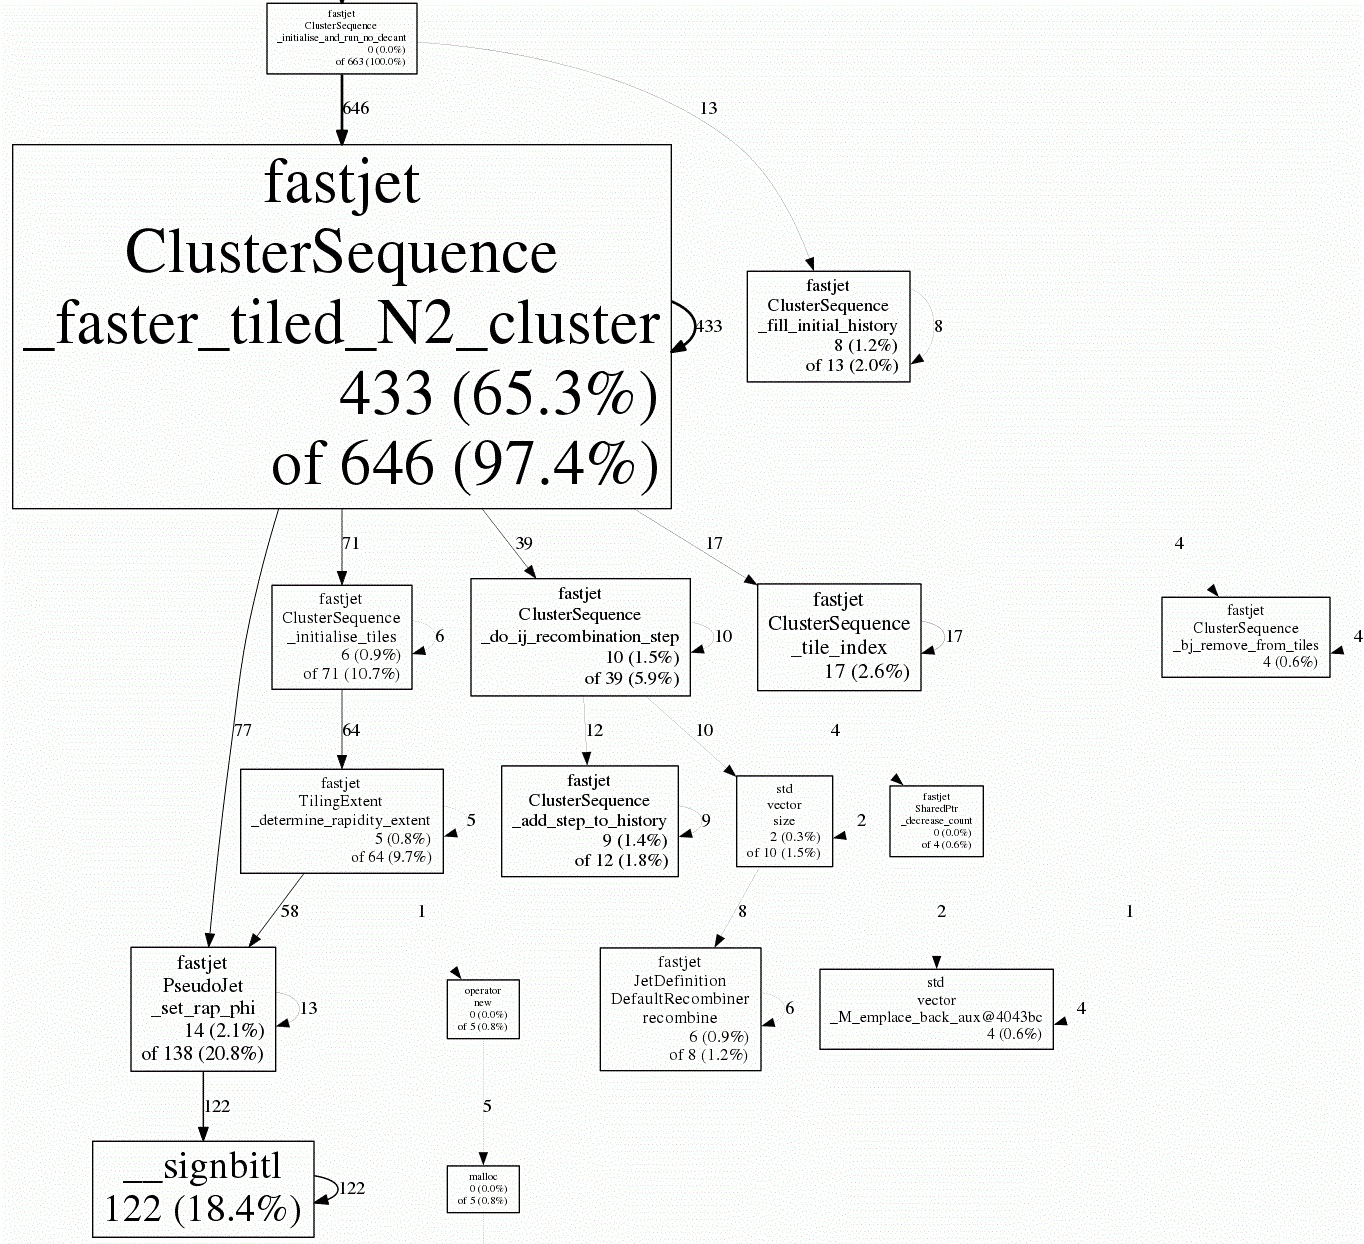
\includegraphics[width=1\linewidth]{images/august2_camb.jpg}
    \caption{Profiling results for the Cambridge algorithm, focused only on the perform\_clustering function.}
    \label{fig:gperfcamb}
\end{figure}

\subsubsection{Discussion} 
Looking at the results, it is clear that both the Cambridge and the anti-$k_t$ reconstruction algorithms make substantial calls to a function called ClusterSequence\_TiledN2. That is the function that calculates the smallest distance between any two particles, as has been discussed on section \ref{ch:seq}. It can also be deduced that the tiled strategy is chosen. FastJet tiled strategy is explained on subsection \ref{ch:tiled}.

A closer look at the code of the computationally expensive function revealed that it consists of a number of loops. The next chosen step was to find which of those loops were the most computationally expensive in that function.

Going back to the output processing with pprof, this time  \verb|--|lines was selected as granularity option. Unfortunately it didn't produce sensible results, as in the output file, there were question marks instead of line numbers. 

In order to solve that, two attempts were made. The first involved compiling the whole software (FastJet libraries and test code) with the -g flag, so that full debugging information would be produced or without any compiler optimisations (O0 flag). For the second attempt, the alternative profiling way of the two discussed on subsection \ref{ch:gerf1} was tried. Neither of them improved the outcome.

Although gperf tools profiler succeeded in pointing out the most expensive function, it was thought better to try another profiler, hoping it would be able to provide line by line results.

\subsection{Intel VTune Performance Analyzer}\label{ch:vtune}
The next choice of profiler was Intel VTune Performance Analyzer\cite{malladi2009using}, a commercial application for software performance analysis, whose goal is to detect performance bottlenecks in an application. Version 17 is already installed on Cirrus. FastJet was installed again using the Intel compiler.

Using the graphical user interface provided by the profiler, a  new analysis was initiated pointing to the executable, and basic hotspots analysis was chosen as a good starting point for the algorithm analysis.

The results were thorough and informative. For example, using the top-down tree tab shows the most computationally expensive functions in descending order. Filtering in on the perform\_clustering function produces the result of figure \ref{fig:vtune1}. The results are in agreement with the previous output of gperf tools. Again, it can be seen that the biggest portion of run-time is spent on the Cluster\_Sequence\_Tiled\_N2 function.

VTune Amplifier is also able to provides the option to show the source code along with information on the percentage of run-time spent in each line. Figure \ref{fig:vtune2} illustrates that. 

\begin{figure}[H]
    \centering
    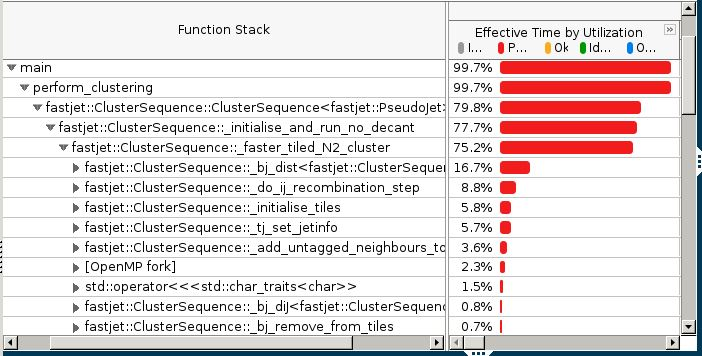
\includegraphics[width=0.9\textwidth]{images/vtune1.JPG}
    \caption{Most computationally expensive functions, from VTune. The results have been filtered in on perform\_clustering function. It can be seen that the most time is spend on the Clsuter\_Sequence\_TiledN2 function.}
    \label{fig:vtune1}
\end{figure}

\begin{figure}[H]
    \centering
    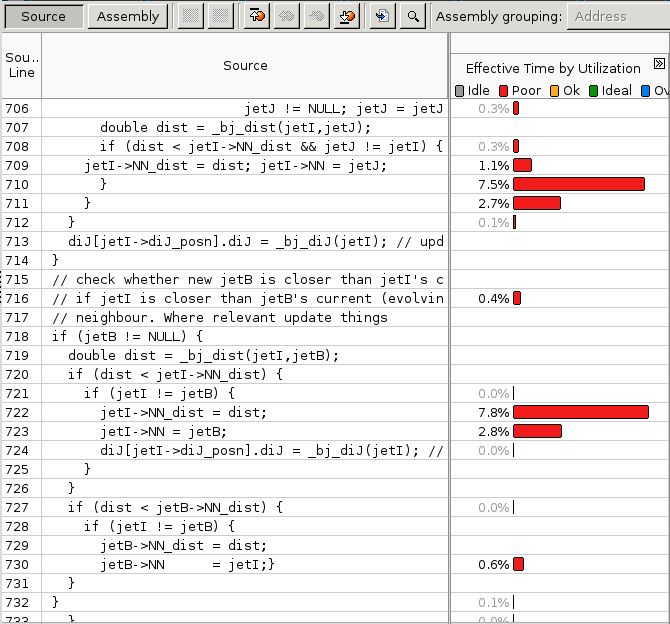
\includegraphics[width=0.85\textwidth]{images/vtune2.JPG}
    \caption{Example result from VTune showing the percentage of run-time spent in each line of source code.}
    \label{fig:vtune2}
\end{figure}

Using the above information, two loops, accounting for 14.2\% (listing \ref{lst:bigishloop}) and 33.3\% (listing \ref{lst:bigloop}) of the clustering time respectively, were pinpointed. Discussion for these loops takes place in the next section.


\section{Discussion of Profiling results}\label{ch:proftalk}
The profiling process revealed that a function called Cluster\_Sequence\_TiledN2, utilising the tiled strategy discussed in section \ref{ch:tiled}, is responsible for the largest proportion of run-time. In it,two loops were identified as the most computationally expensive, accounting for 14.2\% and 33.3\% of the clustering time.

The first of the two most computationally expensive loops is performing part of the set-up for the tiled strategy, and can be seen in listing \ref{lst:bigishloop}.  It loops through all tiles. For every tile, it calculates the nearest neighbour (NN) and nearest neighbour's distance (NN\_dist) of every jet(pseudojet) in the current tile and all tiles to the right side (RH) of it. 

 For each pair of jets processed, the algorithm checks whether the second jet is the nearest neighbour of the first one and whether the first jet is the nearest neighbour of the second. As a result the tiles to the left of each tile do not have to be looped through as they have already been checked.

The second one is responsible for finding the two (developing) jets closest to each other, and is shown in listing \ref{lst:bigloop}. It takes place multiple times per event reconstruction: once per step, until all the particles have been clustered or a stopping criterion has been reached. There are four nested loops. Through every tile, every jet in that tile, all neighbouring tiles, all jets in those tiles. All newly computed distances between jets are registered, and if any of them is smaller than the registered smallest distance, the latter is updated.

For a reminder of what the clustering algorithm calling these two loops does, refer back in sections \ref{ch:seq}, \ref{ch:fjstrategy} and \ref{ch:tiled}. The number of tiles is different for each event, but the average number of tiles that the jets are being separeted into is ten.

\lstinputlisting[language=C++, caption=The second most computationally expensive loop identified that accounts for 14.2 percent of runtime.,label=lst:bigishloop,escapechar=|]{codes/bigish_loop.cc}

\lstinputlisting[language=C++, caption=The most computationally expensive loop identified that accounts for 33.3 percent of runtime.,label=lst:bigloop,escapechar=|]{codes/big_loop.cc}

At that point of the dissertation project, a number of questions were raised. Can those loops be paralelised using OpenMP? If yes, will that aid performance? With some back of the envelope calculations: analysis of each event takes around 100 microseconds. The OpenMP overhead to open a parallel region is between the range of 10-100 microseconds, depending on the system. Things are already not looking too bright in this path.

\section{Efforts to speed-up FastJet}

\subsection{Parallelise over particle events}
Each particle collision event can be worked on individually from the rest. In principle, parallelising over events, providing the workload is enough, should have a near optimal speed-up curve, relative to the number of cores. It was decided that it was worth testing this speculation. To parallelise over events in the test code the loop that calls the Cluster Sequence function was included in a parallel for loop, as can be seen on listing \ref{lst:par_events}.

\begin{lstlisting}[language=c++,caption=Code fraction that parallelised over events,label=lst:par_events,escapechar=|]
int number_of_events = all_events.size();
all_jets.resize(number_of_events);//resize the vector of vectors prior to the loop, so that the reconstructed jets will be placed in the same position as in the serial program.

#pragma omp parallel for schedule(static)
//workload is on average the same for each particle event
//Static scheduling, to avoid the overhead of sharing the workload in an other way
    for(int k=0;k<number_of_events;k++)
    {
        vector <PseudoJet> current_event = all_events[k];

        //for each event run the jet clustering 
        //with the appropriate jet definition        
        ClusterSequence clust_seq(current_event, jet_def);

        //Sort the particles in the jet from larger to smaller momentum.
        //ptmin is the threashold  momentum of particles to filter out of the jet.
        double ptmin = 0;
        vector<PseudoJet> jets = sorted_by_pt(clust_seq.inclusive_jets(ptmin));
        //save the newly reconstructed and sorted jet to the appropriate position fo the vector of vectors
        all_jets[k] = jets;
    }//end of the loop through all events
}
\end{lstlisting}

A subtle point was the sequence in which the reconstructed jets would be saved to the vector. While the output result could still be correct if the jets were stored out of sequence, there was not a way to be certain. Thus, the vector was resized to the appropriate size prior to the loop, and then each thread positioned the reconstructed  jet in the appropriate place.

A static scheduling option was chosen because all the events to be reconstructed needed on average the same computational work. There was no need for a more sophisticated scheduling option that would add extra overhead.

\begin{figure}[H]
    \centering
    \begin{subfigure}{\textwidth}
        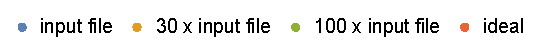
\includegraphics[width=1\linewidth]{images/coarseplotlegend.eps}
    \end{subfigure}
    
    \begin{subfigure}{\textwidth}
        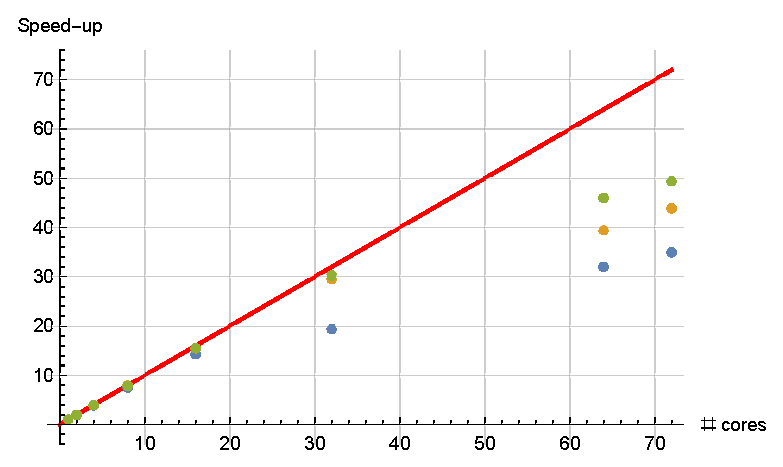
\includegraphics[width=1\linewidth]{images/coarseplot.eps}
    \end{subfigure}
    \caption{fix me: coarse}
    \label{fig:coarse}
\end{figure}

To test the weak scaling, two bigger input files were created, 30 and 100 times the size of input file. Figure \ref{fig:coarse} illustrates the speed-up curve for a different number of threads for the three input files and the ideal speed-up. The bigger the input file, the better the performance, so it can be concluded that workload is the bottleneck for scaling.

\subsection{Parallelising sequential clustering algorithms}

\subsubsection{Pre-existing work}\label{ch:otherswork}

Before proceeding to the work done by the student, in parallelising the clustering algorithms category, it is worth discussing a similar work, performed in \cite{forster2017parallel}. The authors claimed to have succeeded in parallelising the kt algorithm, one of the sequential clustering algorithms used in this project.

After inspecting the work, it was realised that the authors were referring to a non-tiled, obsolete, strategy of the kt algorithm. Although a good starting point, this algorithm has no use in practice, and thus any speed-up gained relative to it has no application. The approach followed was very simplistic, attempting to provide an explanation of the parallelisation process, towards Physicists without a high performance computing background.

Nevertheless, the conclusion of the authors was that, even though the overhead of starting the OpenMP parallel region is bigger than the analysis time for each event, some speed-up was managed to be gained by utilising a thread pool; generating the worker threads only once at the start of the application. That way, the overhead of starting and stopping the threads was minimised.

\subsubsection{Work done by the student}

Following the discussion of section \ref{ch:proftalk}, an attempt to parallelise the most computationally expensive loop (shown in listing \ref{lst:bigloop}) was made. The code fragment was studied to determined any parts of it prone to race conditions. For every pair of jets being looped through, their distance is being calculated locally. This distance is then checked again the global value of the nearest neighbour of the active jet. This part, extending from line \ref{line:crit1start} to \ref{line:crit1end} was put in a critical region.

The whole loop was included in a parallel for with static scheduling clause. The reason the static scheduling was chosen was that, each event requires the same amount of work on average; the extra complexity of a more sophisticated scheduling clause was not needed. Executing the software in parallel produced the correct results but, unsurprisingly, it was much slower than serial. 

Two possible reasons were thought as candidates for the poor performance. The first is that possibly the the critical region is too restrictive. If that is the case, maybe a restructuring of the loop to allow more of the work to be performed out of the parallel region could aid performance. 

The second possible reason is that the overhead of parallelisation is bigger than the performance gain from sharing the workload.

To test the effect of the critical region on performance, the code was run in parallel without it. The output results, as expected, were wrong. Interestingly the run-time only improved slightly, but was still much slower than serial. The critical region is not the major bottleneck in parallelising FastJet; the overhead of parallelisation is.

\subsubsection{Thread pool}
Since the overhead of opening the parallel region has been identified as the major bottleneck, and following the conclusions of subsection \ref{ch:otherswork}, maybe a good idea would be to create a thread pool. This way the overhead of starting and stopping the OpenMP threads would be minimised. Unfortunately during the current work, there was not enough time to test that hypothesis, and will be left for the future.

Also, the openMP is smart enough to do it by itself. Maybe it is tricked though.



\chapter{Adversarial Neural Networks (ANN)}\label{ch:chann}
The second software that has been worked on is a Particle Jet Substructure Adversarial Neural Network, and is discussed in further detail in chapters \ref{ch:jsann} and \ref{ch:analysisjsann}. This chapter aims to explain briefly what a Neural Network is, and the added complexity of it being an adversarial one.

\section{What is a neural network?}

Neural networks are a biologically influenced model, with the aim to learn, recognise patterns, and make decisions in a human-like way. They are used in various applications, ranging from stock market prediction to medical science \cite{ch7nn} and rely on a plain and systematic way of analysing input data. They have achieved considerable success due to today’s recently data availability growth and affordable computational power \cite{nnarticle1}.

%\begin{figure}[H]
%    \centering
\begin{figure}]H]%{0.48\textwidth}
  \centering
  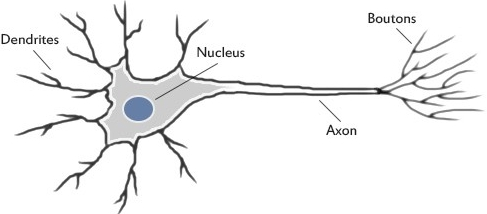
\includegraphics[width=1\textwidth]{images/nn0.jpeg}
  \caption{A neuron in our brain. From \cite{nnarticle2}.}
  \label{fig:realnneuron}
\end{figure}

The human brain uses a network of neurons to process information and model the world around us. A neuron (shown in figure \ref{fig:realnneuron}) collects inputs from other neurons, using dendrites, and sums them. If the resulting value is greater than a threshold, it fires; The signal is then sent to other nearby neurons in the network. 

\begin{figure}[H]%{0.48\textwidth}
  \centering
  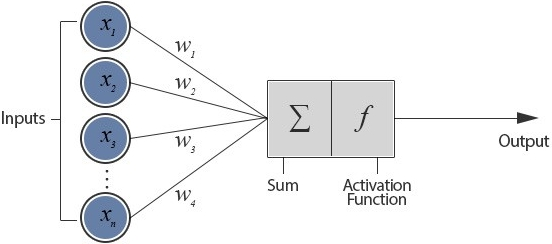
\includegraphics[width=1\textwidth]{images/nn1.jpeg}
  \caption{Model of an artificial neuron (Perceptron). From \cite{nnarticle2}.}
  \label{fig:artifialneuron}
\end{figure}
%\label{neurons}
%\caption{blah blah neurons. From \cite{nnarticle2}}
%\end{figure}


Artificial neural networks mimic that behaviour. As can be seen in figure \ref{fig:artifialneuron}, a neuron is connected with a number of other neurons and receives inputs from them. This configuration is called a Perceptron. 

All the inputs are individually weighted, added together and passed into an activation function. The inputs ($x_i$) and weights ($w_i$) are real numbers and can be positive or negative. The purpose of the activation function is to transform the input signal into an output signal and are necessary for neural networks to model complex non-linear patterns that simpler models might miss. There are many types of activation functions: linear, sigmoid, hyperbolic tangent and more. 

\begin{comment}
There are various options for an activation function but the simplest one is the step function\footnote{A step function will typically output a 1 if the input is higher than a certain threshold, otherwise it’s output will be 0.}.

An example\cite{nnarticle2} would be,
\begin{itemize}[noitemsep]
    \item[] Input 1 ($x_1$) = 0.6, Input 2 ($x_2$) = 1.0
    \item[] 
\end{itemize}
\begin{itemize}[noitemsep]
    \item[] Weight 1 ($w_1$) = 0.5
    \item[] Weight 2 ($w_2$) = 0.8
\end{itemize}
\begin{itemize}[noitemsep]
    \item[] Threshold = 1.0 
\end{itemize}
Weighing the inputs and adding them together gives, 
\begin{itemize}[noitemsep]
\item[]$x_1 * w_1 + x_2 * w_2 = (0.6 * 0.5) + (1 * 0.8) = 1.1$
\end{itemize}

Here, the total input is higher than the threshold and thus the neuron fires. 
\end{comment}

A neural network is created by assembling together many simple perceptrons, so that the output of one of them can be the input of another. For example, figure \ref{fig:simplerernn} shows a small neural network. In this example, the three main parts of a neural network can be identified: the input layer (layer 1), the hidden layer (layer 2), and the output layer (layer 3). The input layer consists of as many perceptrons as there are variables in the input data, while the output layer of as many as the output of the neural network is. The hidden layer is responsible to transform the input data in a way that the output layer can use to reach conclusions.


\begin{figure}[H]
  \centering
  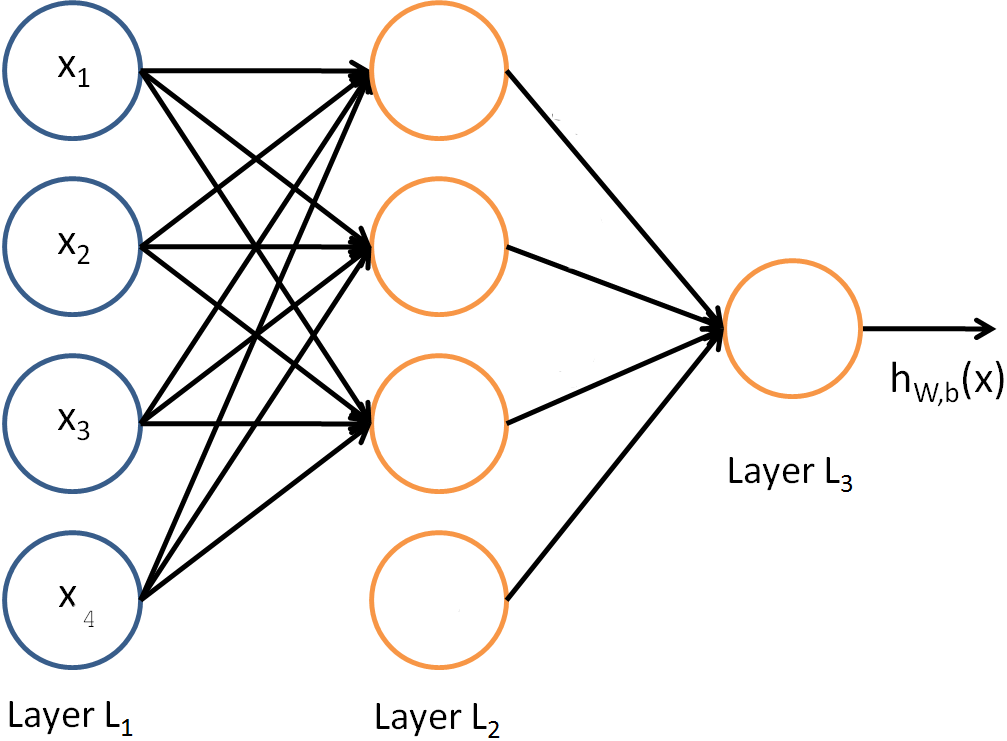
\includegraphics[width=\textwidth]{images/mysimplerernn.png}
  \caption{blah blah blah Taken from \cite{nnarticle3}}
  \label{fig:simplerernn}
\end{figure}

The circles represent neurons and lines represent synapses. Synapses take the input and multiply it by a “weight” (the “strength” of the input in determining the output). 

\section{Training a Neural Network}

For supervised training of a neural network, there should exist training data that have already been classified. This means that for every training input sample, the desired result of the neural network is known. 

The training involves calibrating all of the individual “weights” by repeating two key steps: forward propagation and back propagation. In forward propagation, a set of weights is being applied to the input data and the output is calculated. For the first forward propagation, the set of weights is selected randomly. In back propagation, the margin of error of the output is measured and the weights are adjusted accordingly to decrease the error using an equation.  This equation makes use of a lot of matrix vector multiplications.

Neural networks repeat forward and back propagation until the weights are calibrated to accurately predict an output. When all the training data have passed through the network, an epoch has passed, the network has (possibly) improved in predicting the correct output. Usually more than one epochs are needed for efficient training of the neural network. The loss function is a representative output of how many mistakes the neural network made during a training epoch.

\section{Using a Neural Network}
After the neural network has been trained, it can be used to make predictions in data it has not been trained on. Usually a part of the trained data are being reserved and not included in the training phase, so the neural network can be tested on them.

\section{Multi-layered neural networks}
\begin{figure}[H]
  \centering
  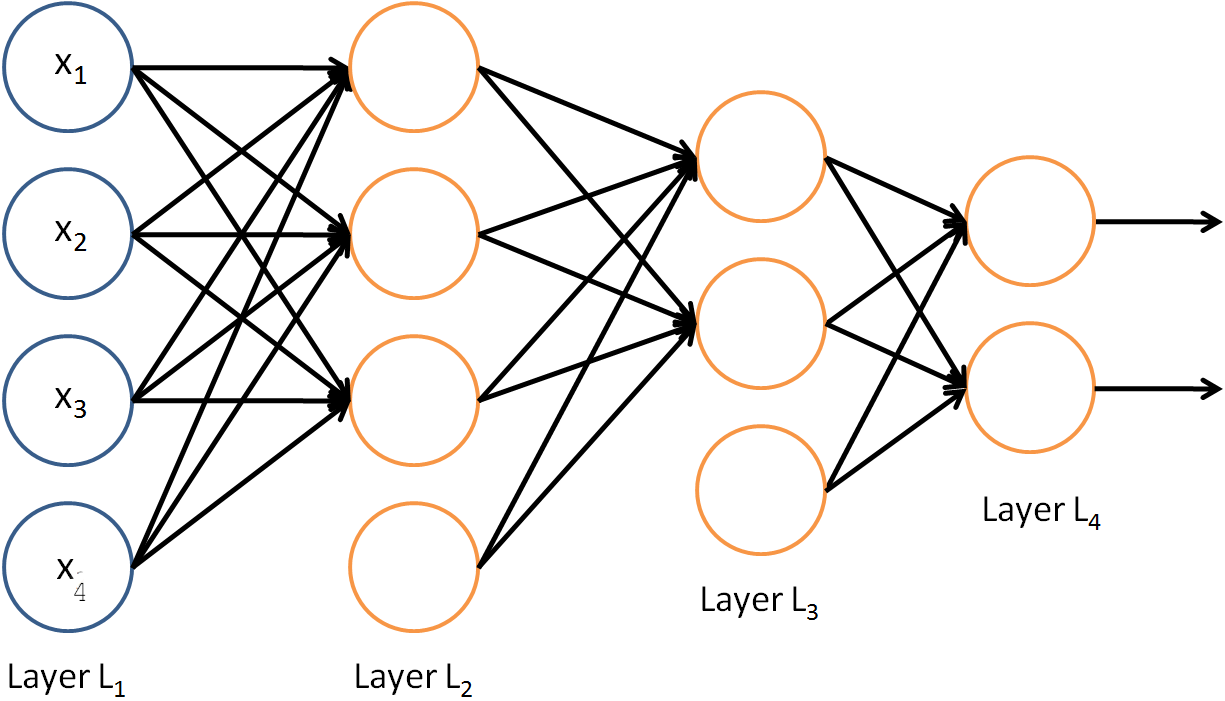
\includegraphics[width=\textwidth]{images/my_simplenn.png}
  \caption{blah blah blah Taken from \cite{nnarticle3}}
  \label{fig:simplenn}
\end{figure}

When the neural network has to make sense of something really complicated, more than one hidden layers are needed (figure \ref{fig:simplenn}) in order to transform the input data into information that the output layer can use to reach conclusions. The term “deep” learning came from having many hidden layers. 


\section{Adversarial Neural Networks}\label{ch:ann}
Adversarial Neural Networks is a recent idea \cite{goodfellow2014generative}, in which two models are trained simultaneously, competing with each other. 
%in a cat and mouse game. 
The first one is a generative model, that is a model whose task is to learn how to create new samples that are as close as possible to the input data.
The second model is what is called an adversary. The goal of the adversary is to determine whether a sample came from the input data or the generative model.

The two models are set in direct opposition. Generative model creates new samples and its adversary try to infer whether those came from the input data or the generative model. Both of them continuously improve from their interaction until a steady stage is reached.

%A generative model is set in direct opposition against an adversary: a discriminative model that learns to determine whether a sample is from the model distribution or the data distribution. 

The generative model can be thought of as analogous to a team of counterfeiters, trying to produce fake currency and use it without detection, while the adversary model is analogous to the police, trying to detect the counterfeit currency. Competition in this game drives both teams to improve their methods until the counterfeits are indistinguishable from the genuine articles \cite{goodfellow2014generative}.

\chapter{The Jet substructure ANN}\label{ch:jsann}
As discussed in section \ref{ch:sub_alg} there exist a category of jet variables representing the probability that a particular jet has substructure or what that substructure may be. All those different variables include some sort of bias though. What if a neural network was trained to take as input the result of those variables, and make an unbiased decision on the matter? 

Turns out that a simple neural network using as input different substructure variables, cannot easily do that. The reason it that many of those variables are dependent from each other, resulting in even the neural network's decision to be biased. 

As a workaround, an adversarial neural network \cite{shimmin2017decorrelated} was created. Essentially, one neural network performs jet substructure classification, while an adversary attempts to guess some properties of the jet solely from the classifier's output. If the adversary was able to guess correctly, it means there was some bias in the classifier's decision, and the latter is penalised. This can be seen in the diagram of figure \ref{fig:achitecture}.

 
\begin{figure}[H]
    \centering
    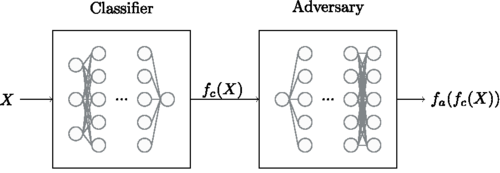
\includegraphics[width=\textwidth]{images/annarchitecture.jpeg}
    \caption{Caption}
    \label{fig:achitecture}
\end{figure}


The input data originate from the substructure algorithms implemented in FastJet, based on simulated data. Thus, it is already known whether those data have substructure or what type it is.


\section{Aspects of the network}

\subsection{The classifier}
The classifier neural network has eleven input variables, three fully connected hidden layers each with 300 nodes, and a single output node. Its inputs are jet substructure variables, similar to jettiness and D2 that were discussed in subsection \ref{ch:sub_alg}.

\subsection{The adversarial}
The adversarial network has a single input node, 50 nodes and an output layer corresponding to the guessed properties of the jet in question.

\subsection{Input data}
The current input file used for training the network, consists of 22 million jets. Each jet takes up 96 bytes of memory, thus the input data file take up around 2GB of memory.

The data set used for experiments is divided into two parts. 80\% of the data are used for training, while the other 10\% for testing. 

\subsection{Training stages}
The training of the jet substructure neural network has three stages. 

Initially the classifier is trained for a number of epochs; typically 200. Then, the adversary is trained for 10 epochs while the classifier is fixed. Finally, the combination of the classifier and the adversary are trained together for another 200 epochs.


\section{Technical characteristics}
Under the hood, the jet substructure adversarial neural network is written in Python and is composed of around 700 thousand lines of code. It makes use of Keras on top of Tensor-flow. 

\subsection{Tensor-flow}
TensorFlow is an open-source framework created by Google for creating Deep Learning models. It allows for instant creation of trained production models and is currently the number one deep learning framework.

No focus will be given on tensor-flow, in this project, as it just serves as the base for Keras.

\subsection{Keras}

Keras \cite{keras} is a high-level neural networks API, able to run on top of TensorFlow. Usually, application writtein using Keras cannot match the speed of neural networks written natively in tensor-flow; the strong weapon of Keras is the simplicity of creating neural networks. In a few lines of code a full working network can be implemented. It is able to run on both CPU and GPU.

\subsubsection{Keras sample code}
\lstinputlisting[language=python, caption=fix me please. Taken from \cite{keras2}.,escapechar=|]{codes/keras.py}

\subsubsection{Batch size}
A Keras parameter that will become important in the next chapter is the batch size. The batch size states the amount of input data that the network should be trained on before the weights are evaluated again. Choosing the optimal batch size value is not an easy task.

In case the batch size is too small, the calculated values have less statistical significance and the weights might jump around. As a result, the neural network converges slower but this way it may be easier to escape any local minimum.

For very big batch size, the network converges much faster but the weights can be stack in local minima and reduce the generalisation ability of the model. For more information, read \cite{keskar2016large}.

In case the neural network is trained on a GPU, the batch size also controls one more technical aspect: the amount of data that will be copied at once to the GPU card. If the batch size is small less data are being copied, which is faster but doesn't keep the kernels busy for much time. For big batch sizes, the kernels have more work to do, per batch delivered, but maybe the whole batch doesn't fit in the GPU card's memory.  


\section{Installation}\label{nninstall}
        The software currently resides in a git repository\cite{anngit} and the project's wiki includes a quick start section. The installation instructions are simple. Clone the git repository and run an installation bash shell script.
        
        Under the hood, the install script, initially installs anaconda, a sandboxed environment for scientific python. In a similar way to the singularity container (discussed on section \ref{ch:singularity}), anaconda provides the ability to create environments that encapsulate a collection of software. 
        
        After the installation of anaconda, the script creates two anaconda environments, for CPU and GPU usage. In each of those environments, a number of software is being installed. The most important of those are Python, Tensor-flow, Keras and CERN Root. The last is a scientific software framework heavily utilised at CERN. The difference between the two environments is that the GPU environment installs a variation of Tensorflow with GPU support. 
    


\section{Usage}\label{nnuse}
        With the software installed, in order to enter the appropriate anaconda environment and load the necessary modules, the user can execute a script
    \begin{lstlisting}
            source activate.sh <<argument>>\end{lstlisting}
        where the argument can either be \textbf{cpu} or \textbf{gpu}, depending whether the user desires GPU support or not. The loaded modules depend on the system.

        A shell script is provided with the source code, that when ran downloads the input file for the software. Afterwards, to execute the software, the following command should be issued
        
        \begin{lstlisting}
python -m run.adversarial.train  <<list of optional arguments>>\end{lstlisting}
        where the arguments (those that will be used during this work) are
        \begin{itemize}
            \item \textbf{--train}\verb|           |Train both the classifier and adversary
            \item \textbf{--train-classifier}\verb|    |Train only the classifier
            \item \textbf{--train-adversarial}\verb|  |Train only the adversary
            \item \textbf{--cpu}\verb|            |Run on CPU (default)
            \item \textbf{--gpu}\verb|            |Run on GPU
            \item \textbf{--devices DEVICES}\verb|  |Number of GPU devices to use (default value is 1)
            \item \textbf{--config CONFIG}\verb|   |The path to the configuration file
            \item \textbf{--help}\verb|            |Show a help message and exit
            \item \textbf{--tensorboard}\verb|      |Use TensorBoard, a visualisation tool for TensorFlow



        \end{itemize}
     
        Note that the training strategy depends in the existence of training results. If the neural network has been trained already, the default strategy is to not train unless forced by an argument.
        
        Appendix \ref{ch:nnoutput} shows the output of the neural network when ran with the \verb|--|train flag. 

\chapter{Performance analysis of the Jet substructure ANN}\label{ch:analysisjsann}


In the first section of this chapter, any difficulties faced while installing the software on different systems are described. Then the first performance experiments are presented, followed by profiling of the code with two different profilers. Finally, some elementary efforts to optimise the performance, based on the conclusions reached from the analysis, are presented.



\section{Installation adventure}

        The procedure described on sections \ref{nninstall} and \ref{nnuse} was followed in order to install and execute the software on the three computing systems mentioned in section \ref{ch:nnwhere}. Although, the installation, for the most part, was smooth, a small number of errors had to be dealt with.
        
        \begin{itemize}
            \item[]\textbf{During installation:}
            \item An old version of SciPy, a scientific python package, was being installed by default. This was causing conflicting dependencies with the other packages and the installation would fail. \\
            To fix that, the installation script was changed so that the latest version of SciPy is being used.
            \item Joblib, a module that aids parallelising loops in Python, was not being installed by the script but was required.\\
            As a fix, the joblib module was added to the installation script.
            \item[]\textbf{On execution:}
            \item The interpreter would complain about a variable that was out of scope and quit.\\
            The bug was fixed by defining the variable in a more appropriate place.
            \item Midway through the project, after cloning the latest commit from the repository, the software stopped working. The reason was that the format of the input file was changed. Thus the existing input file that was supplied to the student became obsolete.\\
            A new input file was provided by the physics department. Also, a new branch to work on was created in the repository to be immune to future software commits by the developing team.  
        \end{itemize}
        

\section{Computing Systems Used}\label{ch:nnwhere}
As the neural network can be run on either CPU or GPU machines, two main systems were chosen, Cirrus and Jade. Also, for quick GPU runs a small system called deeplearn was used.
    \subsection{Cirrus}
    Cirrus was the main system used for CPU performance measurements of the neural network for the same reasons it was chosen for FastJet.
        \subsubsection{Hardware}
        The hardware of Cirrus is discussed in section \ref{ch:cirrus}. 

    \subsection{Jade}
    Jade is the largest GPU facility in the UK. Since access to it was granted for the dissertation, it was used for the GPU performance measurements of the neural network. Being a new system to the student, it took some time to gain familiarity. As the project progressed though, the focus was more and more towards GPU performance. Consequently, most of the results presented in this chapter, come from Jade. 
        \subsubsection{Hardware}
        Jade\cite{jade1} is a UK academic Tier-2 resource and consists of 22 nodes, each containing 8 NVIDIA Tesla P100 GPU cards, linked by NVIDIA's NV link interconnect.  
    
        \subsubsection{Running on the back-end}
        Submitting a job to the back-end of JADE would result to an error about not having permission to do so. A claim was submitted to the technical support team and a few days later the appropriate permissions were granted and the issue was resolved.
        
        The JADE submission script allows the user to chose the desired number of GPU cards to be reserved. Initially, the same number of cards that would be used by the software were also reserved. It was noticed that the timing results were not consistent. This was attributed to the fact that the CPU inside a node cannot be reserved, and could potentially be shared with other users. 
        
        As a solution, every submission script was requested for 8 GPU cards (a whole node), to make sure that the CPU was also reserved. Jobs then, waited in the queue a much longer amount of time, but the timing results were consistent. 
        
    \subsection{Deeplearn}
    The JADE GPU facility is generally very busy. Requesting a whole node for every experiment run would result in wasting a lot of time. To account for that and any time period that Jade would be unavailable, a small system, deeplearn, monitored by EPCC was used. 
    
    Although no results presented in this chapter, originated from deeplearn, the system was extremely helpful for running quick experiments, that did not necessarily have to be ran on Jade. 

    \subsubsection{Hardware}
        Deeplearn consists of an Intel Quad Core 2.40GHz CPU, 8GB of RAM and an NVIDIA GeForce GTX TITAN X graphics card.
        
\section{Does it run on GPU?}
On JADE and Deeplearn, it was not immediately clear that after adding the \verb|--|gpu argument, the training was performed on the GPU cards. Other than the performance being better than from using the \verb|--|cpu argument, nothing else indicated that the training took place on the GPU card.

Since the neural network can output a Tensorboard log file, that file would be use to get an answer. Tensorboard requres port forwarding to visualise the results, which is not allowed in Jade; the firewall seems to be blocking port forwarding. As a workaround, the tensorboard log file was copied to the student's laptop and then visualised. 

After that, Tensorboard worked and provided insightful information regarding the model. Figure \ref{fig:tensorboard2} is a visualisation of the classifier model; the combined model was to complex to present. Even though Tensorboard's result was informational, it didn't succeed in the providing an answer to what whether the GPU cards are being used. The output would read "unknown device". Thus an alternative was sought.

\begin{figure}[H]
    \centering
    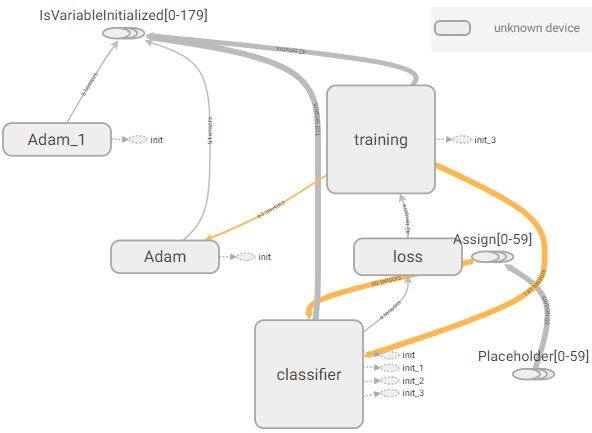
\includegraphics[width=\linewidth]{images/tensorboardgraph1.jpeg}
    \caption{this is wrong. fix me}
    \label{fig:tensorboard2}
\end{figure}


To determine if the GPU cards are being utilised, another strategy was followed. The the neural netwrork was being executed in the background, and the command nvidia-smi was called. This command provides information on the GPU cards existing on the system, like their utilisation, the processes currently using them, their temperature, and more. As can be seen from figure \ref{fig:smi}, the background python code previously executed is using the GPU card, and the utilisation is 25\%. At that point it became clear that the neura network was utilising the GPU cards.
        
        \begin{figure}[H]
            \centering
            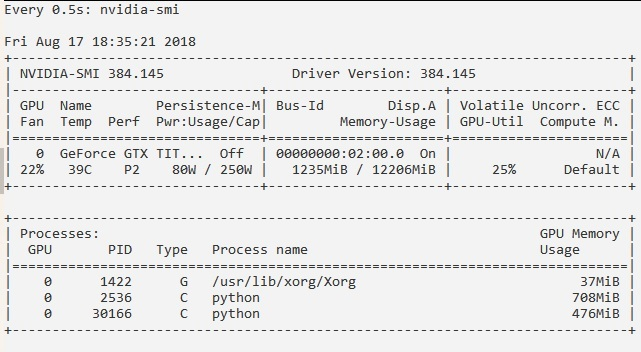
\includegraphics[width=\linewidth]{images/smi2.jpg}
            \caption{fix me: this is smi}
            \label{fig:smi}
        \end{figure}


The reasons for the low utilisation of the GPU cards are discussed further along the way.

\section{Measuring performance}
At that point of the dissertation, the neural network was installed and running on both big systems. It was time for some performance timings; but first the analysis framework should be set up.

\subsection{Performance analysis framework}
All the performance measures presented in this chapter, were run on the back-end of Cirrus if the they were ran on CPU and on the back-end of Jade if they were ran on GPU. 

Unless stated otherwise, timings represent the total run-time for the neural network to trai; this includes the classifier and the combined model. Every measurement presented in this report is the average of 3 runs. 

\subsection{First timing results}
Figure \ref{fig:nn_timings} shows the performance of the neural network on a single Cirrus node (36 CPU cores), and different number of GPU cards from Jade.

Interestingly but not unexpectedly, the performance of the neural network does not improve when more GPU cards are used. If one GPU card is underutilised, how will adding more cards aid performance?


\begin{figure}[H]
    \centering
    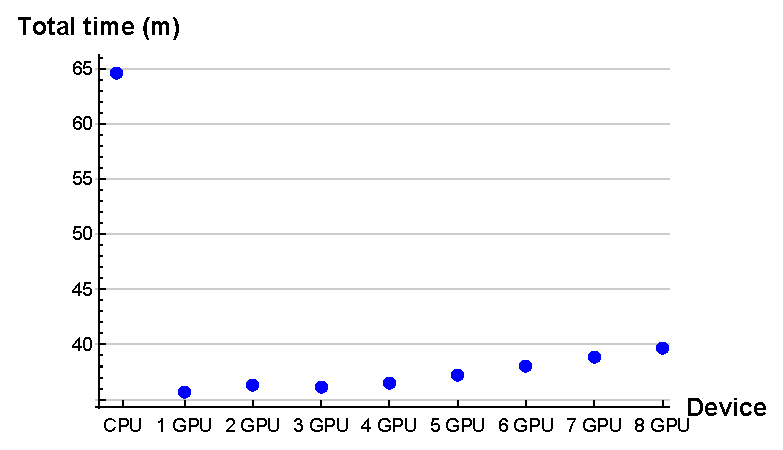
\includegraphics[width=\linewidth]{images/nnperf.eps}
    \caption{Caption:fix me}
    \label{fig:nn_timings}
\end{figure}
 
 
 \section{Profiling}
 \subsection{Vtune Amplifier for CPU profiling}
VTune Aplifier, proved to be a good ally in the performance analysis of FastJet. That was the reason, it was initially used to profile the neural network on Cirrus.

The process was rather trickier this time, as the code is written in python. Python makes use of a runtime interpreter instead of compiling. As a result, there was no binary file of the neural network to select as the executable. 

In order to profile, Python's executable file was selected as the binary to be profiled, and the neural network code was passed as an argument (figure \ref{fig:vtunenn1}).  

\begin{figure}[H]
    \centering
    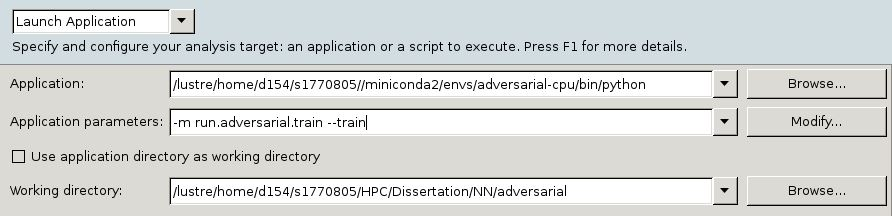
\includegraphics[width=\linewidth]{images/vtunenn.JPG}
    \caption{Caption: fix me}
    \label{fig:vtunenn1}
\end{figure}

This method, succeeded in profiling the code, but the results were in assembly language. As a result, it was hard to reach any conclusions. The physics department was not particularly interested in performance analysis on CPU, thus the effort to profile the neural network on Cirrus was stopped there.

 
 \subsection{NVIDIA Visual Profiler for GPU profiling}
 To profile the neural network on JADE's GPU cards, NVIDIA Visual Profiler (nvprof), that is included with Cuda 9, was used. It was selected because nvprof specialises on the profiling of CUDA applications which is what is going on under the hood of the neural network.
 
 To profile the code on Jade and analyse the results on the students laptop, the instructions for remote profiling in the official documentation\cite{nvprof} were followed. This profiling process included two phases. The first one involved collecting a timeline of the application executing on the remote system, with the least possible intrusion by the profiler. It can be performed with the command 
 \begin{lstlisting}[language=bash]
nvprof --export-profile timeline.prof <app> <app args> \end{lstlisting}

Having done that, the next stage was to collect metrics for the kernels in the application.  This was much more intrusive that the previous phase, and significantly changed the overall performance because all kernel executions were serialised on the GPU. The command for it is
 \begin{lstlisting}[language=bash]
nvprof --metrics achieved_occupancy,executed_ipc -o metrics.prof 
    <app> <app args>\end{lstlisting}

For the second part of the profiling to finish in a reasonable amount of time, the number of epochs was set to 1 and only the classifier was trained. The output files from timeline and metrics were copied locally and opened with nvidia visual profiler. The profiler automatically merges the two results to get an accurate picture of the applications behaviour.

\begin{figure}[H]
    \centering
    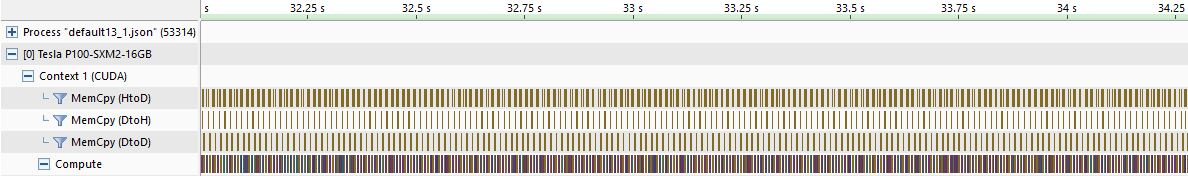
\includegraphics[width=\linewidth]{images/nv13.jpeg}
    \caption{Caption: fix me}
    \label{fig:nvprof1}
\end{figure}

\begin{figure}[H]
    \centering
    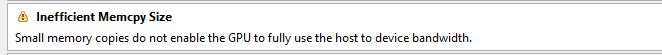
\includegraphics[width=\linewidth]{images/nvwarning.jpeg}
    \caption{Caption: fix me2}
    \label{fig:nvprof2}
\end{figure}



Figure \ref{fig:nvprof1} shows the memory copies from Host (CPU) to the Device (GPU) and vice-versa, and the compute time for 2 representative seconds during the training. It can be seen that the memory copies to the Device are very often but Kernels quickly run out of work. The result of the guided analysis is shown in figure \ref{fig:nvprof2}.   

\textbf{(to do) Understand why 4/8 GPU were slower that one}

 
\section{Attempts made to improve performance}

 \subsection{Optimising data copying by hand}
 One of the goals set at the start of this dissertation was to improve the way data are being fed to the GPU cards. This is currently implemented by Keras calls, but there exists an old commit in the repository with a working simple parallelisation attempt. The plan was to retrieve it, revise it to work with any changes that took place in the meantime, and improve it.
 
That goal was left out for a number of reason. First of all, the commit is pretty old. Thus, a considerable amount of work-time would have to be put solely to make it work with the current state of the software. That is without even considering the time to improve it. Also, following discussions with the developing team, the simplicity and support offered by Keras implementation was preferred to a possible performance gain.

From that point onwards, the attempted optimisations were through Keras.  

\subsection{Tuning the batch size}
To address the under-utilisation of the GPU cards, different values of the bath size were tested to see how this affects performance. The speculation was that, bigger batch sizes would feed the Kernels with more work to do, maybe enough to work until the next batch of data comes.

Figure \ref{fig:batchsize1} show the result. For batch size values smaller than $2^9$ samples, the run-time was more than 10 hours and is not included, while for sizes bigger than $2^{17}$ samples, data would not fit in the memory of the GPU cards. The default value for the batch size is $2^{13}$ samples.

The bigger the batch size, the better the performance. Figure \ref{fig:batchsize2} shows the speed-up curve for different batch sizes. Got a 4x speedup.

It was noticed that altering the batch size affects also the training accuracy of the neural network. The model is less efficient when a bigger batch-size is used. Was the speed-up gained from altering the batch size in vain?


\subsection{Setting a stopping criterion} 
To investigate the relation between the batch size and the training accuracy of the neural network, a stopping criterion was set, instead of the constant 200 epochs. This way, the training would stop once a specific acuracy was reached, an the different batch sized could be compared  on equal terms.

KERAS provides a way to set a stopping criterion, through a function. The arguments of this function are:
\begin{itemize}
    \item \textbf{min\_delta:} minimum change of the loss function to qualify as an improvement.
    \item \textbf{patience:} number of epochs with no improvement after which training will be stopped.
    \item \textbf{baseline:} Baseline value for the monitored quantity to reach. Training will stop if the model doesn't show improvement over the baseline.  
\end{itemize}

Following discussions with the developing team, setting a hard threshold where the training would stop was the best solution, to compare the different batch sizes between them. Thus, baseline value was set to !!!!, patience to zero. 


The stopping criterion was only implemented on the classifier training. That is because, on the adversarial part of the neural network, the two networks are constantly antagonising each other and improving. The way that the combined model's accuracy is improving is not as straightforward.


Figure \ref{fig:criterion1} shows the number of epochs needed to reach the same classification accuracy for different batch sizes.

Figure \ref{fig:criterion2} shows the time needed to reach a classification accuracy for different batch-sizes.

Figure \ref{fig:criterion3} shows the speed-up gained.

(read andreas email)



\chapter{Discussion}
\section{FastJet in the future}

What is likely to change in the near future at experimental particle physics?

More events? More particle per event? More energetic particles?  

Future of experimental particle physics

The same number of proton bunches will be colliding

Each bunch will contain more protons though.

Each event is two bunches colliding. Not two proton.

This means, in the future, we will have the same number of events, but more output particles per event.

Due to having more kinetic energy, the boosted particles will be harder to tag.

Harder to parallelise, because all the jets will be on top of each other. 

Also more particles means that another strategy will be used.

\section{Reflection}


\chapter{Conclusions}
\input{chapters/6-conclusions.tex}

\appendix 
\chapter{Test Code for FastJet}\label{ch:test_code_code}
\lstinputlisting[language=C++]{codes/test_code.cc}

\chapter{NN output}\label{ch:nnoutput}
\lstinputlisting[language=bash, caption=fix me: nnoutput,label=lst:nnoutput,escapechar=|]{codes/nn_output.sh}

%\chapter{Gperf tools results}\label{ch:gperfresults}
%\begin{figure}[H]
    \centering
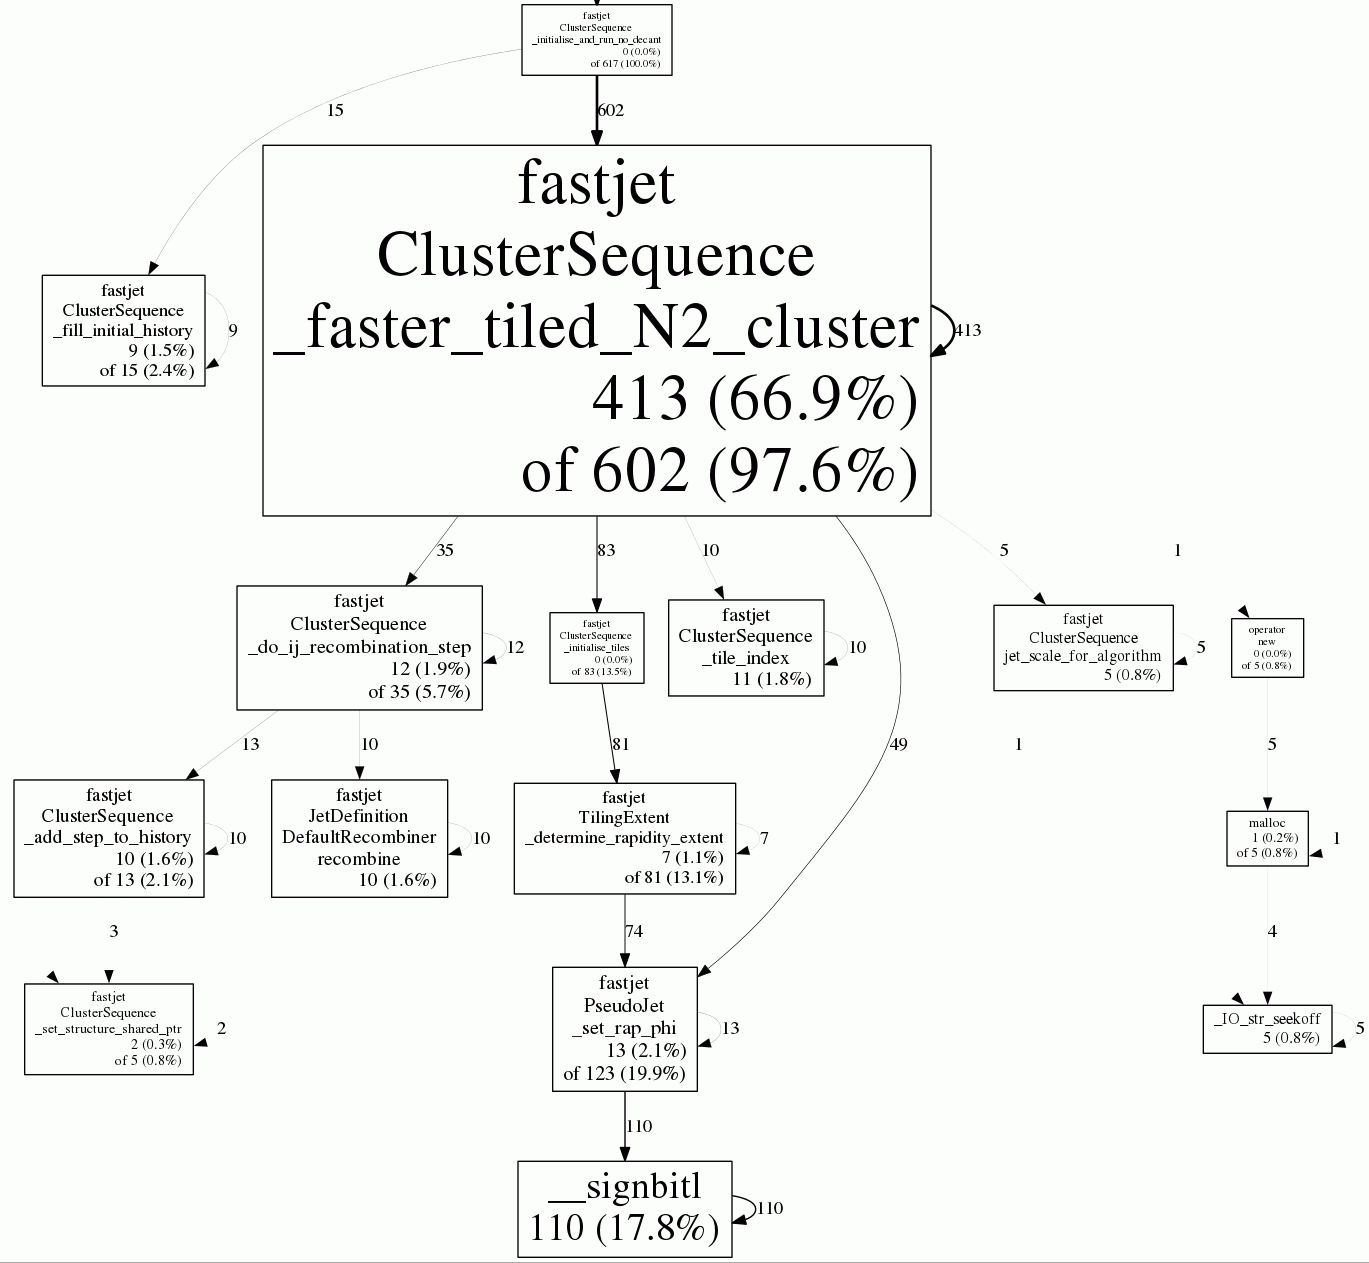
\includegraphics[width=1\linewidth]{august2_antikt.jpeg}
    \caption{Focused profiling results for anti-kt algorithm}
    \label{fig:gperfnatikt}
\end{figure}

\begin{figure}[H]
    \centering
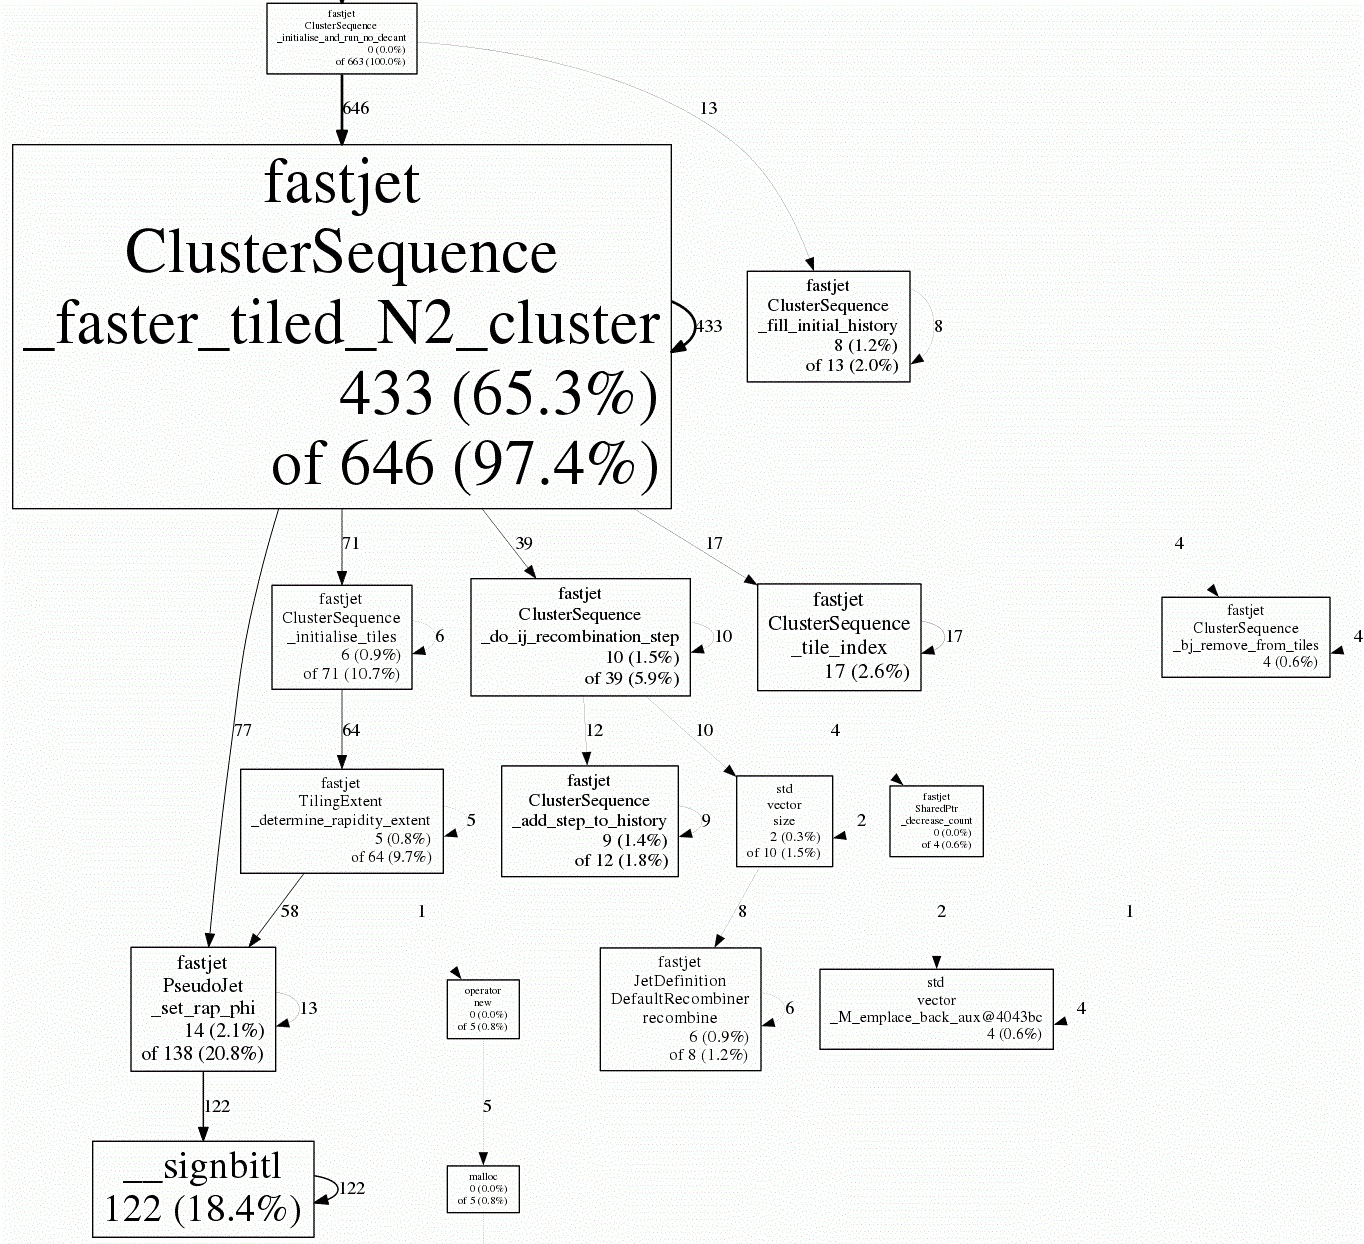
\includegraphics[width=1\linewidth]{images/august2_camb.jpg}
    \caption{Focused profiling results for the Cambridge algorithm}
    \label{fig:gperfcamb}
\end{figure}

\begin{comment}
\end{comment}

\printbibliography
\end{document}

